% ============================================================
% Mục 8. Tính toán / mô phỏng / thực nghiệm  (Đề tài 9)
% Đoạn nội dung (không có preamble): dùng % ============================================================
% Mục 8. Tính toán / mô phỏng / thực nghiệm  (Đề tài 9)
% Đoạn nội dung (không có preamble): dùng % ============================================================
% Mục 8. Tính toán / mô phỏng / thực nghiệm  (Đề tài 9)
% Đoạn nội dung (không có preamble): dùng % ============================================================
% Mục 8. Tính toán / mô phỏng / thực nghiệm  (Đề tài 9)
% Đoạn nội dung (không có preamble): dùng \input{muc8}.
% Cần: amsmath, booktabs, graphicx. Bảng nằm trong generated/ (tự sinh bởi
% make_tables.py từ output/tables), hình nằm trong ../output/figures.
% Chỉ nêu SỐ LIỆU quan sát được; phần diễn giải ý nghĩa thuộc Mục kết quả và phân tích.
% ============================================================
\section{Tính toán, mô phỏng và thực nghiệm}\label{sec:thucnghiem}

\subsection{Cài đặt và kiểm chứng}
Chương trình được viết bằng Python (NumPy, pandas, Matplotlib) và chia thành các tệp
riêng: \texttt{src/model.py} (hai mô hình cầu và các đạo hàm tính tay),
\texttt{src/sensitivity.py} (thay đổi thực, vi phân, sai số, độ nhạy, bậc hội tụ, xấp xỉ
bậc hai, vùng tin cậy), \texttt{src/montecarlo.py} (mô phỏng nhiễu giá),
\texttt{experiments.py} (chạy các thí nghiệm, xuất bảng CSV và hình PNG) và
\texttt{app.py} (ứng dụng tương tác dùng chung mã với báo cáo). Phần mềm chỉ dùng để
tính toán, vẽ đồ thị và kiểm chứng: mọi đạo hàm và công thức sai số được cài đặt từ
các biểu thức ở Mục~\ref{sec:phuongphap}, không gọi hàm có sẵn để tạo kết quả chính.

Việc kiểm chứng do \texttt{verify.py} thực hiện: với $40$ điểm trong miền xác định, các hàm
$q,R,P$ và đạo hàm cấp một, cấp hai cài đặt trong chương trình khớp SymPy với sai lệch
tương đối nhỏ hơn $10^{-9}$, và đạo hàm cấp một khớp sai phân trung tâm với sai lệch
tương đối nhỏ hơn $10^{-5}$; ngoài ra $P'(p^*)=0$ với sai số dưới $10^{-8}$.
Mọi số liệu dưới đây được sinh lại bằng một lệnh (\texttt{uv run experiments.py}) với hạt
giống mô phỏng cố định, nên chạy lại cho kết quả giống hệt.

Tám thí nghiệm (TN) được thực hiện trên hai mô hình ở Bảng~\ref{tab:par}:

\begin{table}[ht]
\tbsty
\caption{Các thí nghiệm và công cụ Giải tích tương ứng.}\label{tab:tn}
\begin{tabular}{@{}l p{6.2cm} p{6.2cm}@{}}
\toprule
TN & Câu hỏi & Công cụ \\
\midrule
1 & Vi phân dự báo thay đổi thực tốt đến đâu? & vi phân, sai số tuyệt đối/tương đối \\
2 & Xấp xỉ tuyến tính trông thế nào? & tiếp tuyến \\
3 & Sai số giảm theo $\Delta p$ với bậc bao nhiêu? & khai triển Taylor, hồi quy log-log \\
4 & Đại lượng nào nhạy nhất với giá? & độ nhạy tương đối $S$ \\
5 & Kết quả có đổi khi đổi tham số mô hình không? & quét $b$ (L) và $k$ (E) \\
6 & Giá nhiễu ngẫu nhiên thì $\Delta P$ phân bố ra sao? & Monte Carlo, Taylor \\
7 & Vi phân dùng được đến mức lệch giá nào? & vùng tin cậy theo ngưỡng $\tau$ \\
8 & Thêm số hạng bậc hai cải thiện bao nhiêu? & xấp xỉ Taylor bậc hai \\
\bottomrule
\end{tabular}
\end{table}

\subsection{TN1: So sánh thay đổi thực và vi phân}
Với mỗi mức lệch $\Delta p/p_0\in\{\pm1,\pm2,\pm5,\pm10,\pm20\}\%$ ta tính $\Delta P$ thực,
$dP=P'(p_0)\Delta p$ và sai số (Bảng~\ref{tab:tn1l} và~\ref{tab:tn1e}; đơn vị của $\Delta P$,
$dP$ là nghìn đồng/tuần).

\begin{table}[ht]
\tbsty
\caption{Lợi nhuận $P$ tại $p_0=50$, mô hình (L).}\label{tab:tn1l}
\input{generated/tn1_linear}
\end{table}

\begin{table}[ht]
\tbsty
\caption{Lợi nhuận $P$ tại $p_0=40$, mô hình (E).}\label{tab:tn1e}
\input{generated/tn1_elastic}
\end{table}

Ở mô hình (L), $E_{\mathrm{rel}}$ tăng từ $1{,}0\%$ ($\Delta p/p_0=\pm1\%$) lên $5{,}3\%$
($+5\%$) và $25{,}0\%$ ($+20\%$); ở mô hình (E) từ $2{,}5\%$ lên $13{,}1\%$ và $60{,}0\%$. Với
(L), $P$ là hàm bậc hai nên $|\Delta P-dP|=\tfrac12|P''|\Delta p^2$ đối xứng giữa hai phía
(ví dụ $62{,}5$ cho cả $\pm5\%$), còn $E_{\mathrm{rel}}$ không đối xứng ($4{,}76\%$ và $5{,}26\%$)
vì $\Delta P$ ở hai phía khác nhau.

Tại giá tối ưu $p^*$ (với $P'(p^*)=0$) thì $dP=0$; thay đổi thực khi giá tăng $5\%$ là
$-140{,}6$ (mô hình L, $p^*=75$) và $-18{,}9$ (mô hình E, $p^*=60$), nên $E_{\mathrm{rel}}=100\%$.
Với $q$ và $R$, kết quả tương tự được lưu trong \texttt{output/tables/}.

\subsection{TN2: Tiếp tuyến và đường cong}
Hình~\ref{fig:tn2l} và~\ref{fig:tn2e} vẽ $q,R,P$ cùng tiếp tuyến tại $p_0$; dải tô màu là
$p_0\pm20\%$. Khoảng cách giữa đường cong và tiếp tuyến chính là sai số của xấp xỉ vi phân,
nhỏ gần $p_0$ và tăng nhanh khi ra xa.

\begin{figure}[ht]
\centering
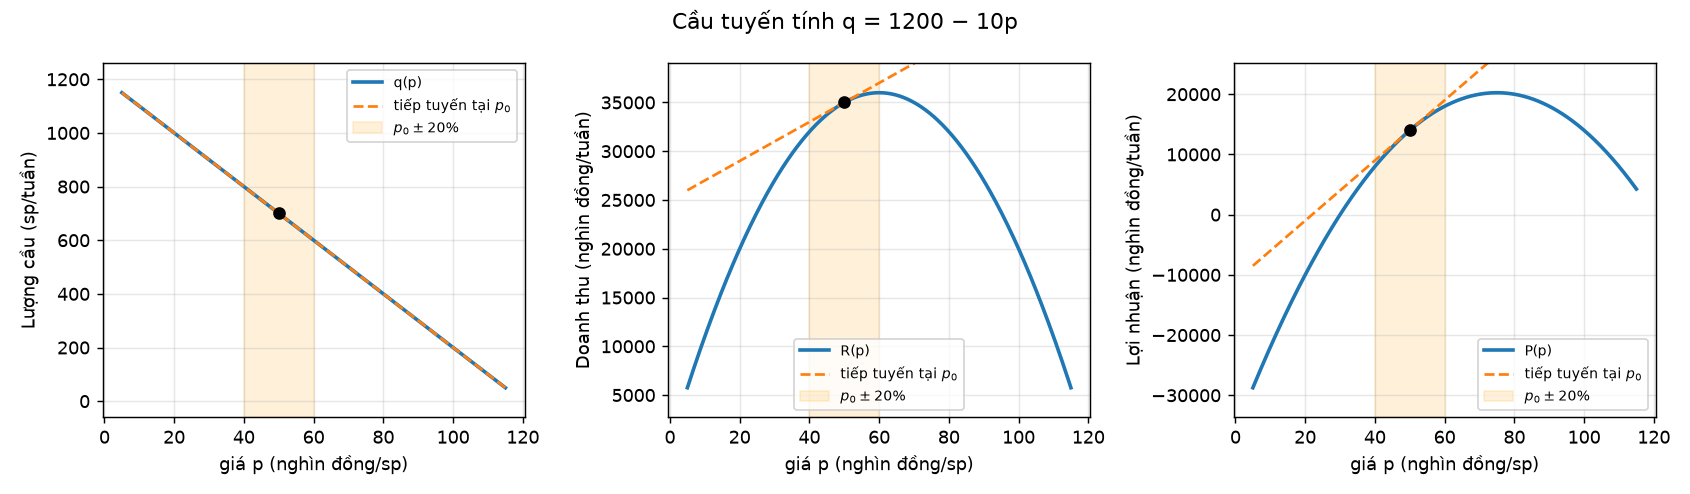
\includegraphics[width=\textwidth]{TN2_tangent_linear.png}
\caption{Mô hình (L): $q$, $R$, $P$ và tiếp tuyến tại $p_0=50$.}\label{fig:tn2l}
\end{figure}
\begin{figure}[ht]
\centering
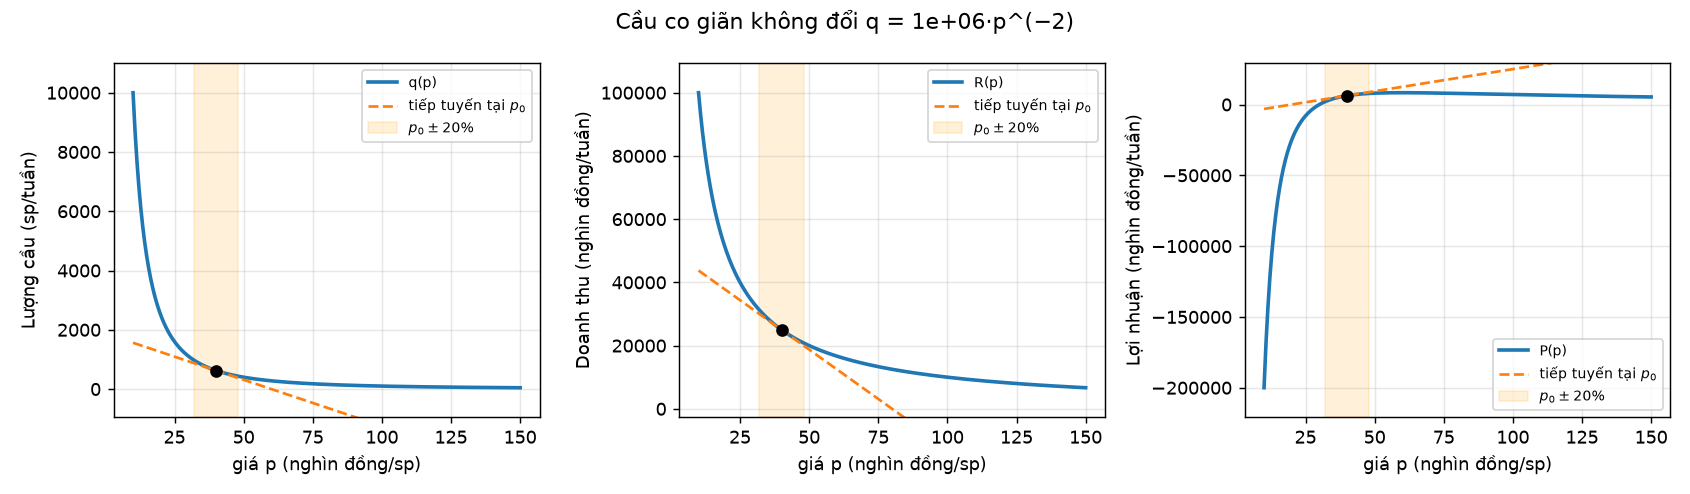
\includegraphics[width=\textwidth]{TN2_tangent_elastic.png}
\caption{Mô hình (E): $q$, $R$, $P$ và tiếp tuyến tại $p_0=40$.}\label{fig:tn2e}
\end{figure}

\subsection{TN3: Bậc của sai số}
Hệ số góc log-log của $E_{\mathrm{abs}}$ theo $|\Delta p|$ (cách đo ở Mục~\ref{sec:phuongphap}) cho trong
Bảng~\ref{tab:tn3}; kỳ vọng là $2$.

\begin{table}[ht]
\tbsty
\caption{Hệ số góc log-log của sai số vi phân. Dấu ``---'': sai số bằng $0$.}\label{tab:tn3}
\input{generated/tn3}
\end{table}

Ở (L), $R$ và $P$ cho đúng $2{,}000$, còn $q$ là hàm tuyến tính nên sai số bằng $0$. Ở (E), các
hệ số góc nằm trong khoảng $1{,}96$ đến $1{,}98$, gần $2$ nhưng hơi lệch vì lưới $\Delta p$ trải đến
$30\%$ nên các số hạng bậc cao bắt đầu có ảnh hưởng (Hình~\ref{fig:tn3}).

\begin{figure}[ht]
\centering
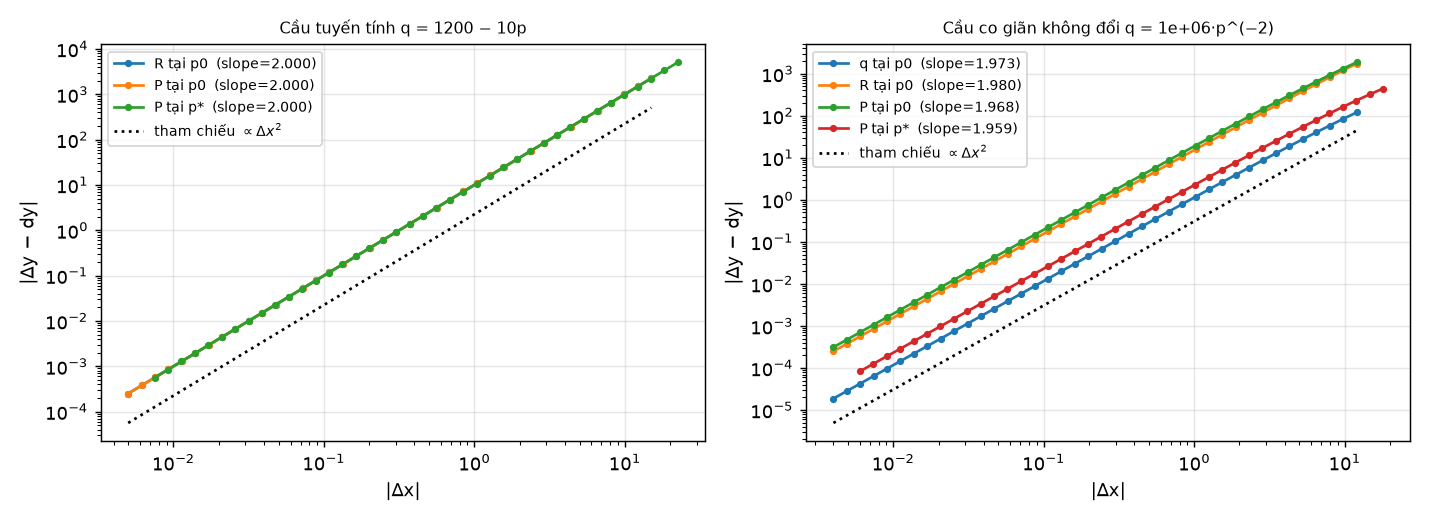
\includegraphics[width=\textwidth]{TN3_error_loglog.png}
\caption{Sai số $|\Delta y-dy|$ theo $|\Delta p|$ (thang log-log) và đường tham chiếu $\propto\Delta p^2$.}\label{fig:tn3}
\end{figure}

\subsection{TN4: Độ nhạy tương đối}
Bảng~\ref{tab:tn4} cho $S=f'p/f$ tại $p_0$ và $p^*$; Hình~\ref{fig:tn4} vẽ $S(p)$ (cắt ở $|S|>12$).

\begin{table}[ht]
\tbsty
\caption{Độ nhạy tương đối của $q$, $R$, $P$ theo giá.}\label{tab:tn4}
\input{generated/tn4}
\end{table}

Tại $p_0$, ở (L) $|S_P|=1{,}786$ lớn nhất, sau đó là $|S_q|=0{,}714$ và $|S_R|=0{,}286$; ở (E)
$S_q=-2$, $S_R=-1$, $S_P=2$, trong đó $|S_P|$ và $|S_q|$ bằng nhau. Các giá trị khớp với hệ
thức~\eqref{eq:S}: ví dụ ở (L), $S_P=50/20-0{,}714=1{,}786$; ở (E), $S_P=40/10-2=2$. Tại $p^*$,
$S_P=0$ ở cả hai mô hình.

\begin{figure}[ht]
\centering
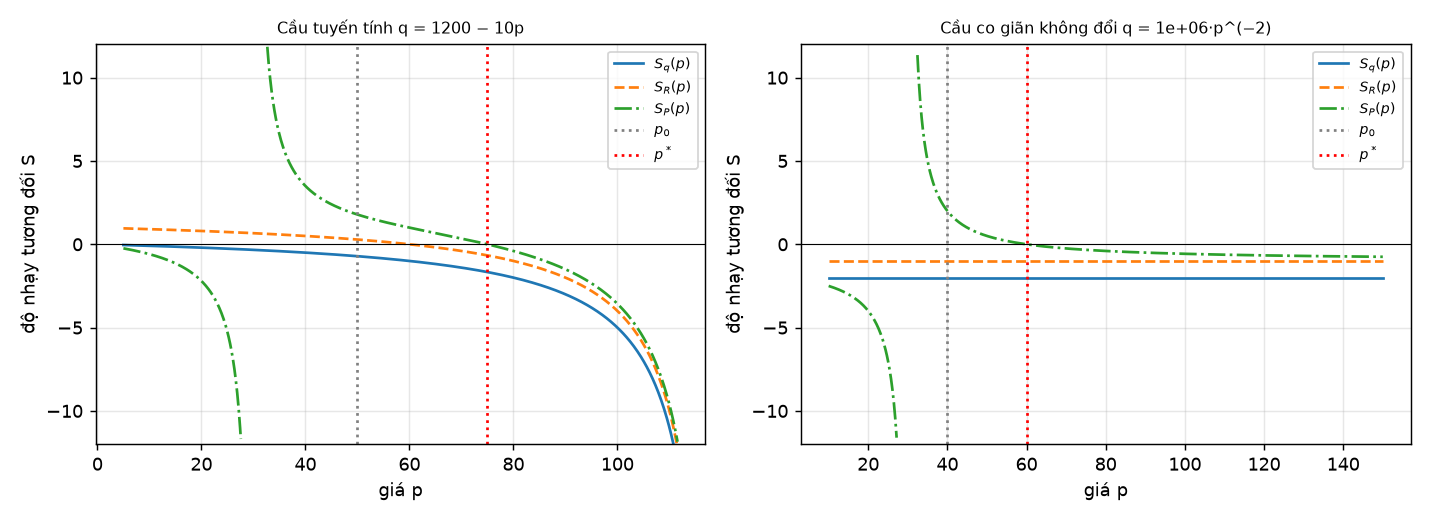
\includegraphics[width=\textwidth]{TN4_elasticity.png}
\caption{Độ nhạy $S_q$, $S_R$, $S_P$ theo giá $p$ (đường chấm: $p_0$ và $p^*$).}\label{fig:tn4}
\end{figure}

\subsection{TN5: Ảnh hưởng của tham số mô hình}
Cố định $\Delta p=+10\%$ và thay đổi độ dốc cầu $b$ (mô hình L) hoặc độ co giãn $k$ (mô hình E); các
bảng cho $E_{\mathrm{rel}}$ của $q$, $R$, $P$.

\begin{center}
\linespread{1}\small\selectfont
\begin{minipage}[t]{0.48\textwidth}\centering
\captionof{table}{Mô hình (L): $E_{\mathrm{rel}}$ (\%) khi thay đổi $b$.}\label{tab:tn5l}
\input{generated/tn5_linear}
\end{minipage}\hfill
\begin{minipage}[t]{0.48\textwidth}\centering
\captionof{table}{Mô hình (E): $E_{\mathrm{rel}}$ (\%) khi thay đổi $k$.}\label{tab:tn5e}
\input{generated/tn5_elastic}
\end{minipage}
\end{center}

\begin{figure}[ht]
\centering
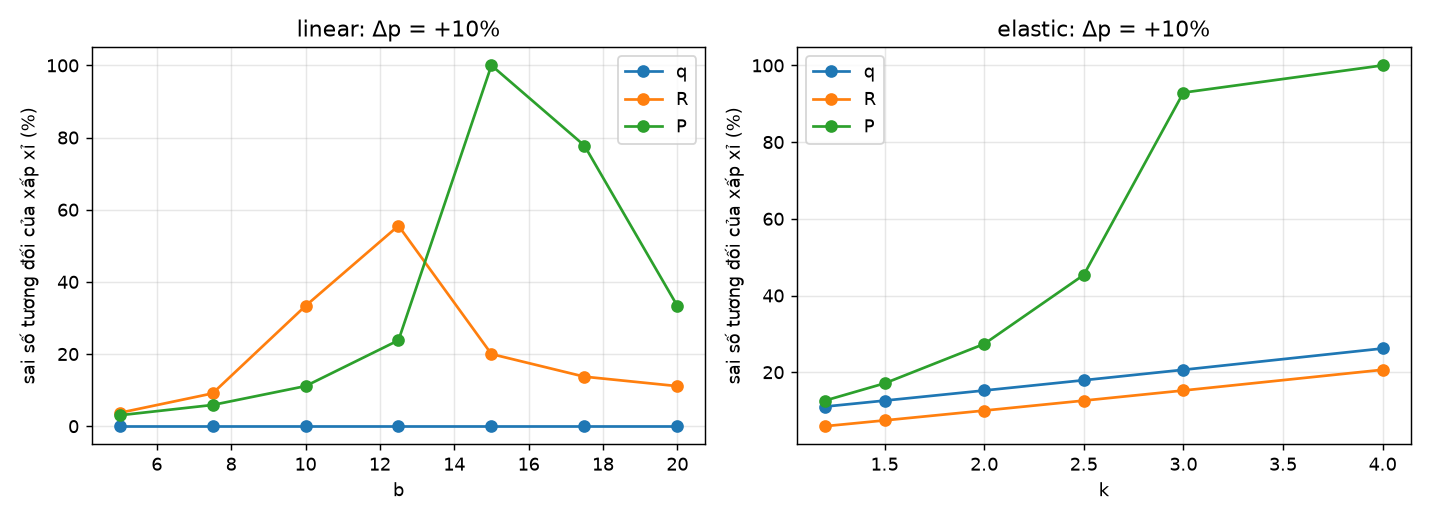
\includegraphics[width=\textwidth]{TN5_param_study.png}
\caption{Sai số tương đối của xấp xỉ vi phân khi $\Delta p=+10\%$ theo tham số mô hình.}\label{fig:tn5}
\end{figure}

Ở (L), $q$ luôn có sai số $0$. Sai số của $P$ không đơn điệu theo $b$: nó đạt $100\%$ tại $b=15$, vì khi
đó $p^*=(a+bc)/(2b)=55$ đúng bằng giá mới $p_0+10\%$, nên $\Delta P=dP/2$. Sai số của $R$ lớn nhất ở
$b=12{,}5$, gần $b=12$ là lúc $R'(p_0)=a-2bp_0=0$. Ở (E), sai số của cả ba đại lượng tăng theo $k$;
$P$ đạt $100\%$ tại $k=4$ vì khi đó $p^*=ck/(k-1)=40=p_0$, tức $P'(p_0)=0$ và $dP=0$.

\subsection{TN6: Mô phỏng Monte Carlo}
Giá thực tế $p=p_0(1+\varepsilon)$, $\varepsilon\sim N(0,\sigma^2)$, $N=200\,000$ mẫu, hạt giống
$20260503$. Bảng~\ref{tab:tn6} so sánh trung bình và độ lệch chuẩn của $\Delta P$ với
dự đoán~\eqref{eq:mc} (đơn vị nghìn đồng/tuần); Hình~\ref{fig:tn6} là phân bố của $\Delta P$ ở mô hình (L)
với $\sigma=10\%$.

\begin{table}[ht]
\tbsty
\caption{Monte Carlo: $\Delta P$ thực và dự đoán từ khai triển Taylor.}\label{tab:tn6}
{\setlength{\tabcolsep}{5pt}\input{generated/tn6}}
\end{table}

Tại $p_0$, độ lệch chuẩn mô phỏng sát dự đoán $|P'|p_0\sigma$ (ví dụ $248{,}5$ so với $250{,}0$ ở (L),
$\sigma=1\%$), và trung bình âm sát $\tfrac12P''(p_0\sigma)^2$; độ lệch tăng khi $\sigma$ lớn ở mô
hình (E) ($1\,499$ so với $1\,250$ khi $\sigma=10\%$). Tại $p^*$ dự đoán bậc nhất của độ lệch chuẩn
bằng $0$ nhưng mô phỏng cho giá trị dương và trung bình âm, phù hợp với $\Delta P\approx\tfrac12P''(p^*\varepsilon)^2\le0$:
với $\sigma=5\%$, công thức $|P''|(p^*\sigma)^2/\sqrt2$ cho $198{,}9$ (L) và $29{,}5$ (E), so với $196{,}2$ và
$31{,}5$ mô phỏng.

\begin{figure}[ht]
\centering
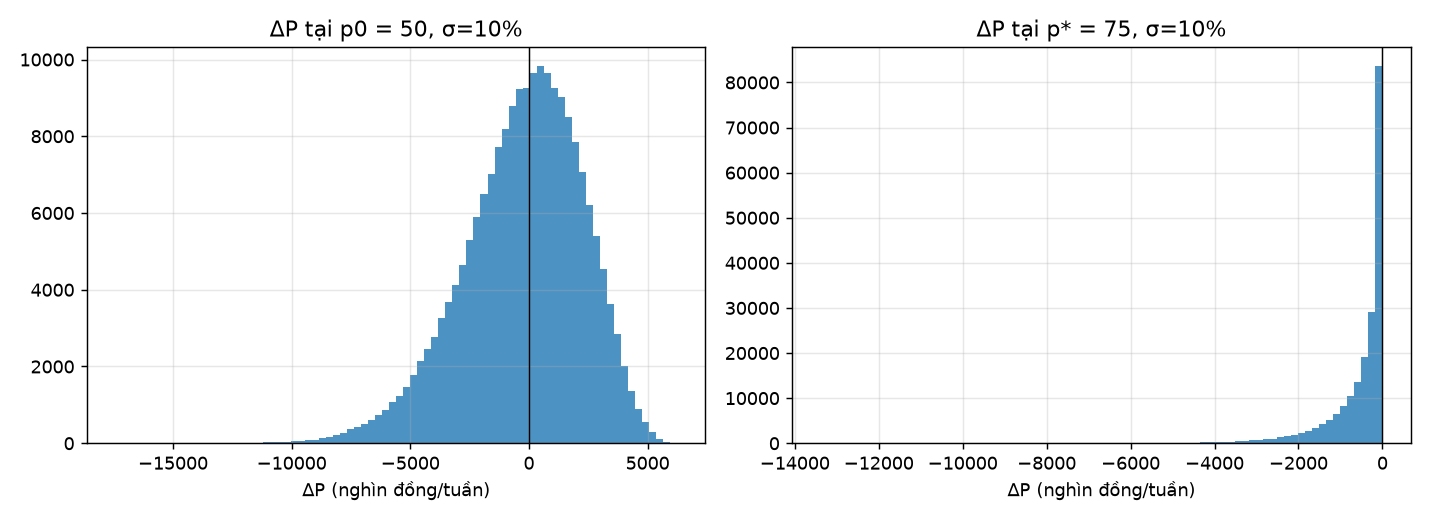
\includegraphics[width=\textwidth]{TN6_montecarlo_hist.png}
\caption{Phân bố của $\Delta P$ ở mô hình (L), $\sigma=10\%$: tại $p_0$ (trái) và tại $p^*$ (phải).}\label{fig:tn6}
\end{figure}

\subsection{TN7: Vùng tin cậy của vi phân}
Bảng~\ref{tab:tn7} cho mức lệch giá lớn nhất (tính theo $\%$ của $p_0$, dạng ``tăng\,/\,giảm'') để
$E_{\mathrm{rel}}\le\tau$; ``$\geq 50$'' nghĩa là không chạm ngưỡng trong khoảng khảo sát.

\begin{table}[ht]
\tbsty
\caption{Vùng tin cậy của vi phân (đơn vị: $\%$ của $p_0$).}\label{tab:tn7}
\input{generated/tn7}
\end{table}

Vùng tin cậy tăng xấp xỉ tỉ lệ với $\tau$ (ví dụ $P$ ở (L): $0{,}95$; $4{,}75$; $9{,}05$ cho $\tau=1;5;10\%$),
đúng như ước lượng~\eqref{eq:safe}. Với cùng $\tau=5\%$, ở (L) $R$ có vùng hẹp nhất ($+1{,}90/-2{,}10$)
còn $q$ chính xác tuyệt đối, trong khi ở (E) $P$ hẹp nhất ($+1{,}95/-2{,}00$). Tại $p^*$ vùng bằng $0$.

\begin{figure}[ht]
\centering
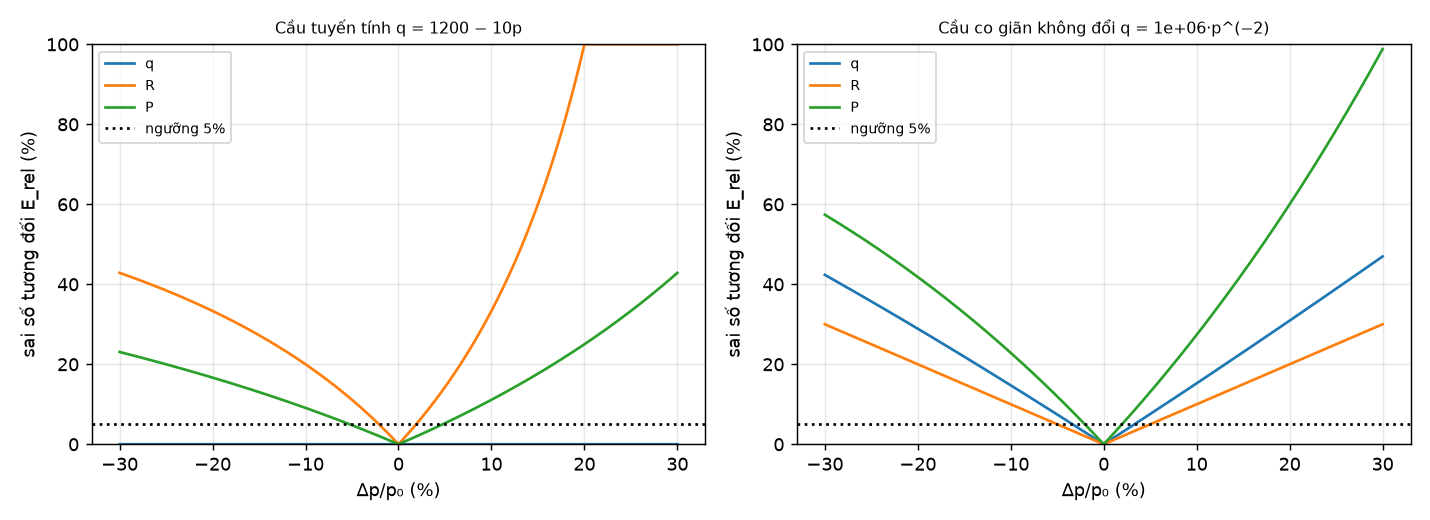
\includegraphics[width=\textwidth]{TN7_erel_vs_delta.png}
\caption{$E_{\mathrm{rel}}$ theo $\Delta p/p_0$ tại $p_0$ (đường chấm: ngưỡng $5\%$).}\label{fig:tn7}
\end{figure}

\subsection{TN8: Xấp xỉ bậc hai}
Bảng~\ref{tab:tn8} so sánh vi phân bậc một $dP$ và xấp xỉ bậc hai $dP_2$ cho $P$ ở mô hình (E).
Ở mô hình (L), $R$ và $P$ là đa thức bậc hai nên $dP_2$ trùng $\Delta P$ ở mọi dòng (sai số $0$).

\begin{table}[ht]
\tbsty
\caption{Mô hình (E): $P$ tại $p_0=40$ và $p^*=60$, xấp xỉ bậc một và bậc hai.}\label{tab:tn8}
{\setlength{\tabcolsep}{5pt}\input{generated/tn8_elastic}}
\end{table}

Tại $p_0$ với $\Delta p/p_0=+5\%$, $E_{\mathrm{rel}}$ giảm từ $13{,}08\%$ xuống $1{,}06\%$; với $+10\%$ từ
$27{,}37\%$ xuống $4{,}47\%$; với $+20\%$ từ $60{,}00\%$ xuống $20{,}00\%$. Tại $p^*$, vi phân bậc một cho
$dP=0$ ($E_{\mathrm{rel}}=100\%$) còn $dP_2$ bắt được thay đổi thực với sai số $10{,}25\%$ ($+5\%$) và
$9{,}75\%$ ($-5\%$). Hệ số góc log-log (Bảng~\ref{tab:tn8o}, Hình~\ref{fig:tn8}) xấp xỉ $2$ cho bậc một và
xấp xỉ $3$ cho bậc hai ($2{,}95$ đến $2{,}96$ ở mô hình E), khớp với lý thuyết ở Mục~\ref{sec:phuongphap}.

\begin{table}[ht]
\tbsty
\caption{Hệ số góc log-log của sai số xấp xỉ bậc một và bậc hai. Dấu ``---'': sai số bằng $0$.}\label{tab:tn8o}
\input{generated/tn8_orders}
\end{table}

\begin{figure}[ht]
\centering
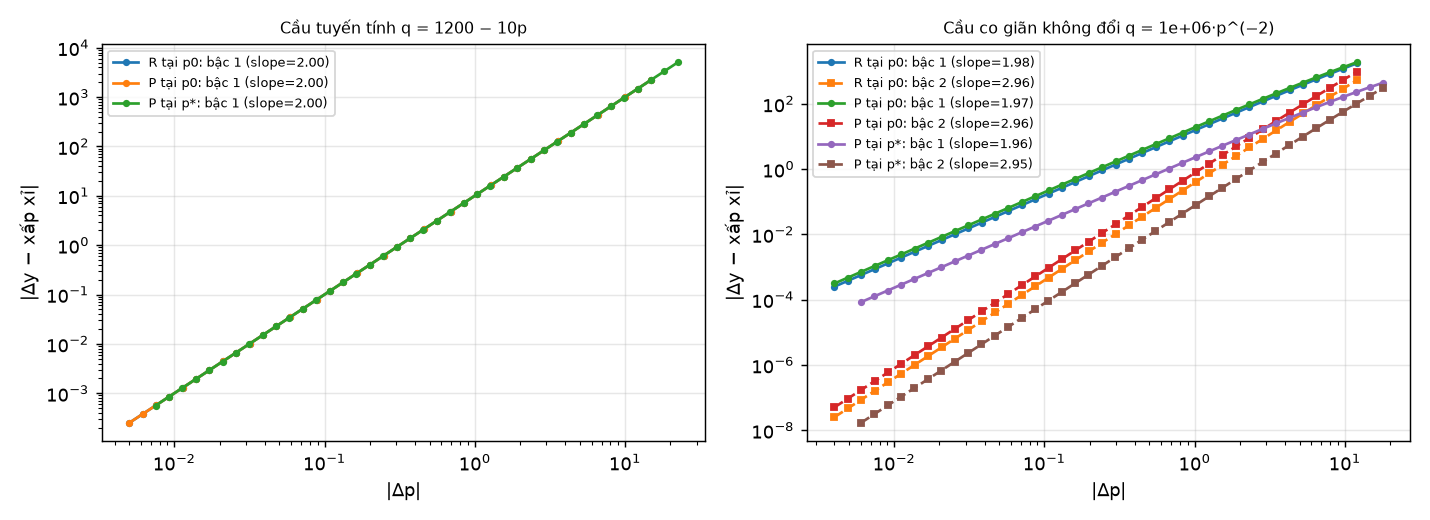
\includegraphics[width=\textwidth]{TN8_second_order_loglog.png}
\caption{Sai số của xấp xỉ bậc một và bậc hai theo $|\Delta p|$ (log-log).}\label{fig:tn8}
\end{figure}
.
% Cần: amsmath, booktabs, graphicx. Bảng nằm trong generated/ (tự sinh bởi
% make_tables.py từ output/tables), hình nằm trong ../output/figures.
% Chỉ nêu SỐ LIỆU quan sát được; phần diễn giải ý nghĩa thuộc Mục kết quả và phân tích.
% ============================================================
\section{Tính toán, mô phỏng và thực nghiệm}\label{sec:thucnghiem}

\subsection{Cài đặt và kiểm chứng}
Chương trình được viết bằng Python (NumPy, pandas, Matplotlib) và chia thành các tệp
riêng: \texttt{src/model.py} (hai mô hình cầu và các đạo hàm tính tay),
\texttt{src/sensitivity.py} (thay đổi thực, vi phân, sai số, độ nhạy, bậc hội tụ, xấp xỉ
bậc hai, vùng tin cậy), \texttt{src/montecarlo.py} (mô phỏng nhiễu giá),
\texttt{experiments.py} (chạy các thí nghiệm, xuất bảng CSV và hình PNG) và
\texttt{app.py} (ứng dụng tương tác dùng chung mã với báo cáo). Phần mềm chỉ dùng để
tính toán, vẽ đồ thị và kiểm chứng: mọi đạo hàm và công thức sai số được cài đặt từ
các biểu thức ở Mục~\ref{sec:phuongphap}, không gọi hàm có sẵn để tạo kết quả chính.

Việc kiểm chứng do \texttt{verify.py} thực hiện: với $40$ điểm trong miền xác định, các hàm
$q,R,P$ và đạo hàm cấp một, cấp hai cài đặt trong chương trình khớp SymPy với sai lệch
tương đối nhỏ hơn $10^{-9}$, và đạo hàm cấp một khớp sai phân trung tâm với sai lệch
tương đối nhỏ hơn $10^{-5}$; ngoài ra $P'(p^*)=0$ với sai số dưới $10^{-8}$.
Mọi số liệu dưới đây được sinh lại bằng một lệnh (\texttt{uv run experiments.py}) với hạt
giống mô phỏng cố định, nên chạy lại cho kết quả giống hệt.

Tám thí nghiệm (TN) được thực hiện trên hai mô hình ở Bảng~\ref{tab:par}:

\begin{table}[ht]
\tbsty
\caption{Các thí nghiệm và công cụ Giải tích tương ứng.}\label{tab:tn}
\begin{tabular}{@{}l p{6.2cm} p{6.2cm}@{}}
\toprule
TN & Câu hỏi & Công cụ \\
\midrule
1 & Vi phân dự báo thay đổi thực tốt đến đâu? & vi phân, sai số tuyệt đối/tương đối \\
2 & Xấp xỉ tuyến tính trông thế nào? & tiếp tuyến \\
3 & Sai số giảm theo $\Delta p$ với bậc bao nhiêu? & khai triển Taylor, hồi quy log-log \\
4 & Đại lượng nào nhạy nhất với giá? & độ nhạy tương đối $S$ \\
5 & Kết quả có đổi khi đổi tham số mô hình không? & quét $b$ (L) và $k$ (E) \\
6 & Giá nhiễu ngẫu nhiên thì $\Delta P$ phân bố ra sao? & Monte Carlo, Taylor \\
7 & Vi phân dùng được đến mức lệch giá nào? & vùng tin cậy theo ngưỡng $\tau$ \\
8 & Thêm số hạng bậc hai cải thiện bao nhiêu? & xấp xỉ Taylor bậc hai \\
\bottomrule
\end{tabular}
\end{table}

\subsection{TN1: So sánh thay đổi thực và vi phân}
Với mỗi mức lệch $\Delta p/p_0\in\{\pm1,\pm2,\pm5,\pm10,\pm20\}\%$ ta tính $\Delta P$ thực,
$dP=P'(p_0)\Delta p$ và sai số (Bảng~\ref{tab:tn1l} và~\ref{tab:tn1e}; đơn vị của $\Delta P$,
$dP$ là nghìn đồng/tuần).

\begin{table}[ht]
\tbsty
\caption{Lợi nhuận $P$ tại $p_0=50$, mô hình (L).}\label{tab:tn1l}
% Tự sinh bởi make_tables.py - không sửa tay.

\begin{tabular}{@{}rrrrr@{}}
\toprule
$\Delta p/p_0$ (\%) & $\Delta P$ thực & $dP$ & $|\Delta P-dP|$ & $E_{\mathrm{rel}}$ (\%) \\
\midrule
${-}20$ & ${-}6\,000{,}0$ & ${-}5\,000{,}0$ & $1\,000{,}0$ & $16{,}67$ \\
${-}10$ & ${-}2\,750{,}0$ & ${-}2\,500{,}0$ & $250{,}0$ & $9{,}09$ \\
${-}5$ & ${-}1\,312{,}5$ & ${-}1\,250{,}0$ & $62{,}5$ & $4{,}76$ \\
${-}2$ & ${-}510{,}0$ & ${-}500{,}0$ & $10{,}0$ & $1{,}96$ \\
${-}1$ & ${-}252{,}5$ & ${-}250{,}0$ & $2{,}5$ & $0{,}99$ \\
${+}1$ & $247{,}5$ & $250{,}0$ & $2{,}5$ & $1{,}01$ \\
${+}2$ & $490{,}0$ & $500{,}0$ & $10{,}0$ & $2{,}04$ \\
${+}5$ & $1\,187{,}5$ & $1\,250{,}0$ & $62{,}5$ & $5{,}26$ \\
${+}10$ & $2\,250{,}0$ & $2\,500{,}0$ & $250{,}0$ & $11{,}11$ \\
${+}20$ & $4\,000{,}0$ & $5\,000{,}0$ & $1\,000{,}0$ & $25{,}00$ \\
\bottomrule
\end{tabular}

\end{table}

\begin{table}[ht]
\tbsty
\caption{Lợi nhuận $P$ tại $p_0=40$, mô hình (E).}\label{tab:tn1e}
% Tự sinh bởi make_tables.py - không sửa tay.

\begin{tabular}{@{}rrrrr@{}}
\toprule
$\Delta p/p_0$ (\%) & $\Delta P$ thực & $dP$ & $|\Delta P-dP|$ & $E_{\mathrm{rel}}$ (\%) \\
\midrule
${-}20$ & ${-}4\,296{,}9$ & ${-}2\,500{,}0$ & $1\,796{,}9$ & $41{,}82$ \\
${-}10$ & ${-}1\,620{,}4$ & ${-}1\,250{,}0$ & $370{,}4$ & $22{,}86$ \\
${-}5$ & ${-}709{,}8$ & ${-}625{,}0$ & $84{,}8$ & $11{,}95$ \\
${-}2$ & ${-}262{,}9$ & ${-}250{,}0$ & $12{,}9$ & $4{,}91$ \\
${-}1$ & ${-}128{,}2$ & ${-}125{,}0$ & $3{,}2$ & $2{,}48$ \\
${+}1$ & $121{,}9$ & $125{,}0$ & $3{,}1$ & $2{,}52$ \\
${+}2$ & $237{,}9$ & $250{,}0$ & $12{,}1$ & $5{,}09$ \\
${+}5$ & $552{,}7$ & $625{,}0$ & $72{,}3$ & $13{,}08$ \\
${+}10$ & $981{,}4$ & $1\,250{,}0$ & $268{,}6$ & $27{,}37$ \\
${+}20$ & $1\,562{,}5$ & $2\,500{,}0$ & $937{,}5$ & $60{,}00$ \\
\bottomrule
\end{tabular}

\end{table}

Ở mô hình (L), $E_{\mathrm{rel}}$ tăng từ $1{,}0\%$ ($\Delta p/p_0=\pm1\%$) lên $5{,}3\%$
($+5\%$) và $25{,}0\%$ ($+20\%$); ở mô hình (E) từ $2{,}5\%$ lên $13{,}1\%$ và $60{,}0\%$. Với
(L), $P$ là hàm bậc hai nên $|\Delta P-dP|=\tfrac12|P''|\Delta p^2$ đối xứng giữa hai phía
(ví dụ $62{,}5$ cho cả $\pm5\%$), còn $E_{\mathrm{rel}}$ không đối xứng ($4{,}76\%$ và $5{,}26\%$)
vì $\Delta P$ ở hai phía khác nhau.

Tại giá tối ưu $p^*$ (với $P'(p^*)=0$) thì $dP=0$; thay đổi thực khi giá tăng $5\%$ là
$-140{,}6$ (mô hình L, $p^*=75$) và $-18{,}9$ (mô hình E, $p^*=60$), nên $E_{\mathrm{rel}}=100\%$.
Với $q$ và $R$, kết quả tương tự được lưu trong \texttt{output/tables/}.

\subsection{TN2: Tiếp tuyến và đường cong}
Hình~\ref{fig:tn2l} và~\ref{fig:tn2e} vẽ $q,R,P$ cùng tiếp tuyến tại $p_0$; dải tô màu là
$p_0\pm20\%$. Khoảng cách giữa đường cong và tiếp tuyến chính là sai số của xấp xỉ vi phân,
nhỏ gần $p_0$ và tăng nhanh khi ra xa.

\begin{figure}[ht]
\centering
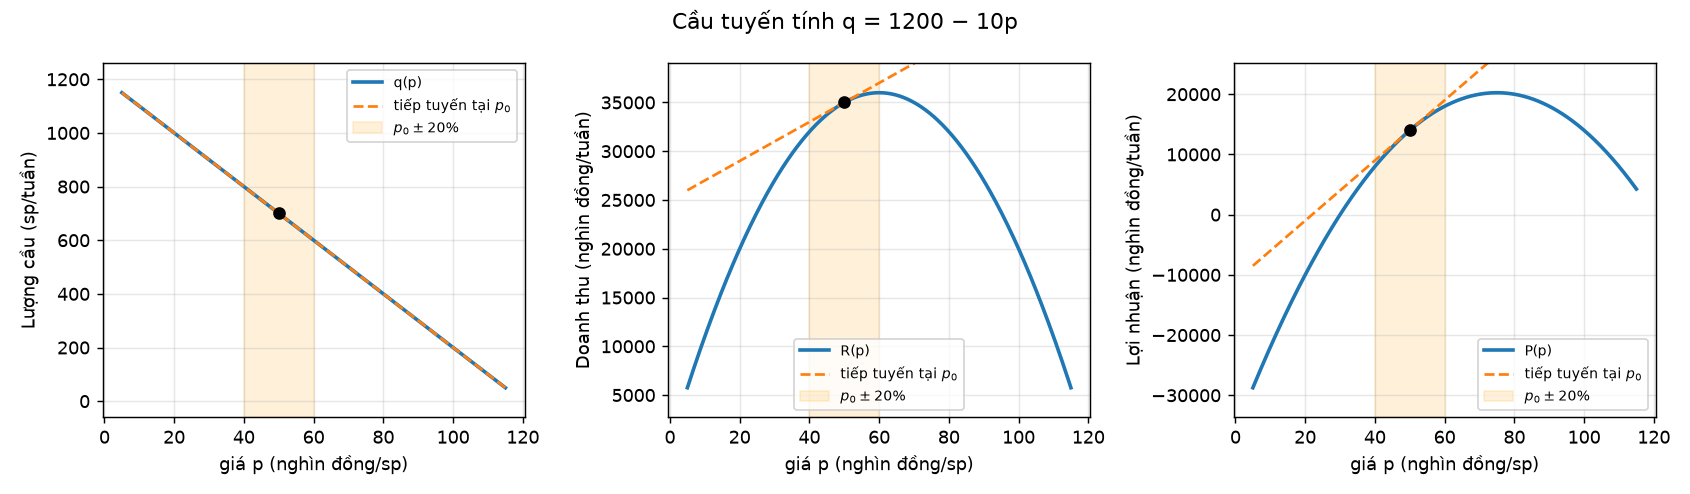
\includegraphics[width=\textwidth]{TN2_tangent_linear.png}
\caption{Mô hình (L): $q$, $R$, $P$ và tiếp tuyến tại $p_0=50$.}\label{fig:tn2l}
\end{figure}
\begin{figure}[ht]
\centering
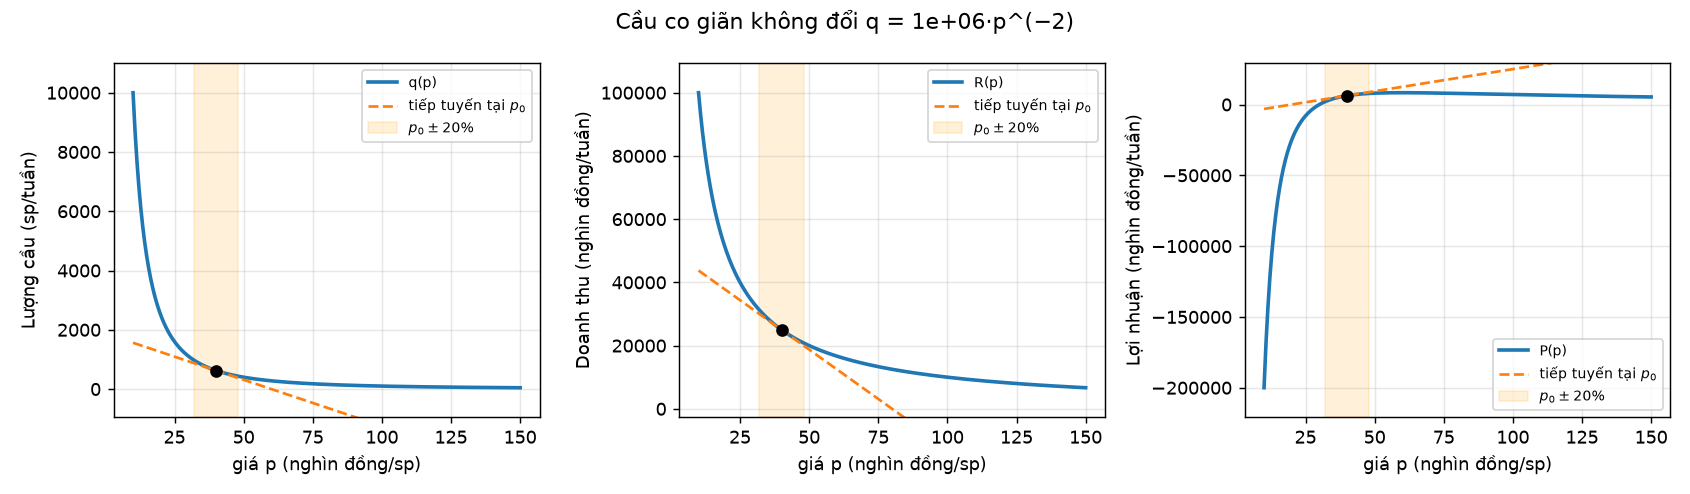
\includegraphics[width=\textwidth]{TN2_tangent_elastic.png}
\caption{Mô hình (E): $q$, $R$, $P$ và tiếp tuyến tại $p_0=40$.}\label{fig:tn2e}
\end{figure}

\subsection{TN3: Bậc của sai số}
Hệ số góc log-log của $E_{\mathrm{abs}}$ theo $|\Delta p|$ (cách đo ở Mục~\ref{sec:phuongphap}) cho trong
Bảng~\ref{tab:tn3}; kỳ vọng là $2$.

\begin{table}[ht]
\tbsty
\caption{Hệ số góc log-log của sai số vi phân. Dấu ``---'': sai số bằng $0$.}\label{tab:tn3}
% Tự sinh bởi make_tables.py - không sửa tay.

\begin{tabular}{@{}llcr@{}}
\toprule
Mô hình & Đại lượng & Điểm & Hệ số góc log-log \\
\midrule
Tuyến tính (L) & $q$ & $p_0$ & --- \\
 & $R$ & $p_0$ & $2{,}000$ \\
 & $P$ & $p_0$ & $2{,}000$ \\
 & $P$ & $p^*$ & $2{,}000$ \\
\midrule
Co giãn (E) & $q$ & $p_0$ & $1{,}973$ \\
 & $R$ & $p_0$ & $1{,}980$ \\
 & $P$ & $p_0$ & $1{,}968$ \\
 & $P$ & $p^*$ & $1{,}959$ \\
\bottomrule
\end{tabular}

\end{table}

Ở (L), $R$ và $P$ cho đúng $2{,}000$, còn $q$ là hàm tuyến tính nên sai số bằng $0$. Ở (E), các
hệ số góc nằm trong khoảng $1{,}96$ đến $1{,}98$, gần $2$ nhưng hơi lệch vì lưới $\Delta p$ trải đến
$30\%$ nên các số hạng bậc cao bắt đầu có ảnh hưởng (Hình~\ref{fig:tn3}).

\begin{figure}[ht]
\centering
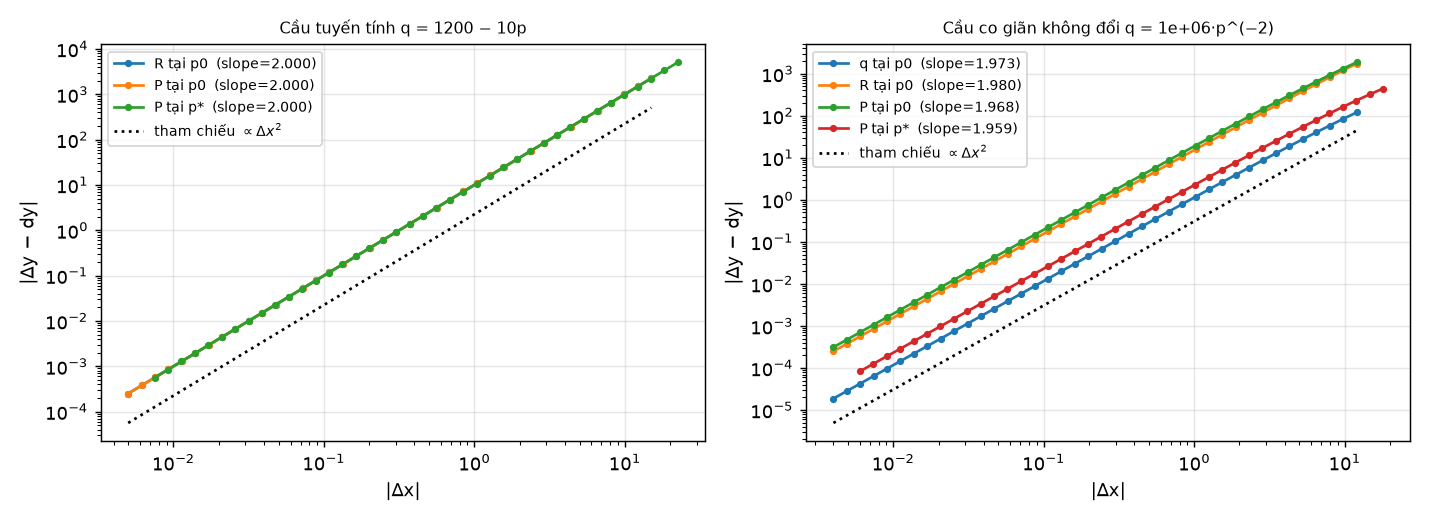
\includegraphics[width=\textwidth]{TN3_error_loglog.png}
\caption{Sai số $|\Delta y-dy|$ theo $|\Delta p|$ (thang log-log) và đường tham chiếu $\propto\Delta p^2$.}\label{fig:tn3}
\end{figure}

\subsection{TN4: Độ nhạy tương đối}
Bảng~\ref{tab:tn4} cho $S=f'p/f$ tại $p_0$ và $p^*$; Hình~\ref{fig:tn4} vẽ $S(p)$ (cắt ở $|S|>12$).

\begin{table}[ht]
\tbsty
\caption{Độ nhạy tương đối của $q$, $R$, $P$ theo giá.}\label{tab:tn4}
% Tự sinh bởi make_tables.py - không sửa tay.

\begin{tabular}{@{}llrr@{}}
\toprule
Mô hình & Độ nhạy & tại $p_0$ & tại $p^*$ \\
\midrule
Tuyến tính (L) & $S_q$ & ${-}0{,}714$ & ${-}1{,}667$ \\
 & $S_R$ & $0{,}286$ & ${-}0{,}667$ \\
 & $S_P$ & $1{,}786$ & $0{,}000$ \\
\midrule
Co giãn (E) & $S_q$ & ${-}2{,}000$ & ${-}2{,}000$ \\
 & $S_R$ & ${-}1{,}000$ & ${-}1{,}000$ \\
 & $S_P$ & $2{,}000$ & $0{,}000$ \\
\bottomrule
\end{tabular}

\end{table}

Tại $p_0$, ở (L) $|S_P|=1{,}786$ lớn nhất, sau đó là $|S_q|=0{,}714$ và $|S_R|=0{,}286$; ở (E)
$S_q=-2$, $S_R=-1$, $S_P=2$, trong đó $|S_P|$ và $|S_q|$ bằng nhau. Các giá trị khớp với hệ
thức~\eqref{eq:S}: ví dụ ở (L), $S_P=50/20-0{,}714=1{,}786$; ở (E), $S_P=40/10-2=2$. Tại $p^*$,
$S_P=0$ ở cả hai mô hình.

\begin{figure}[ht]
\centering
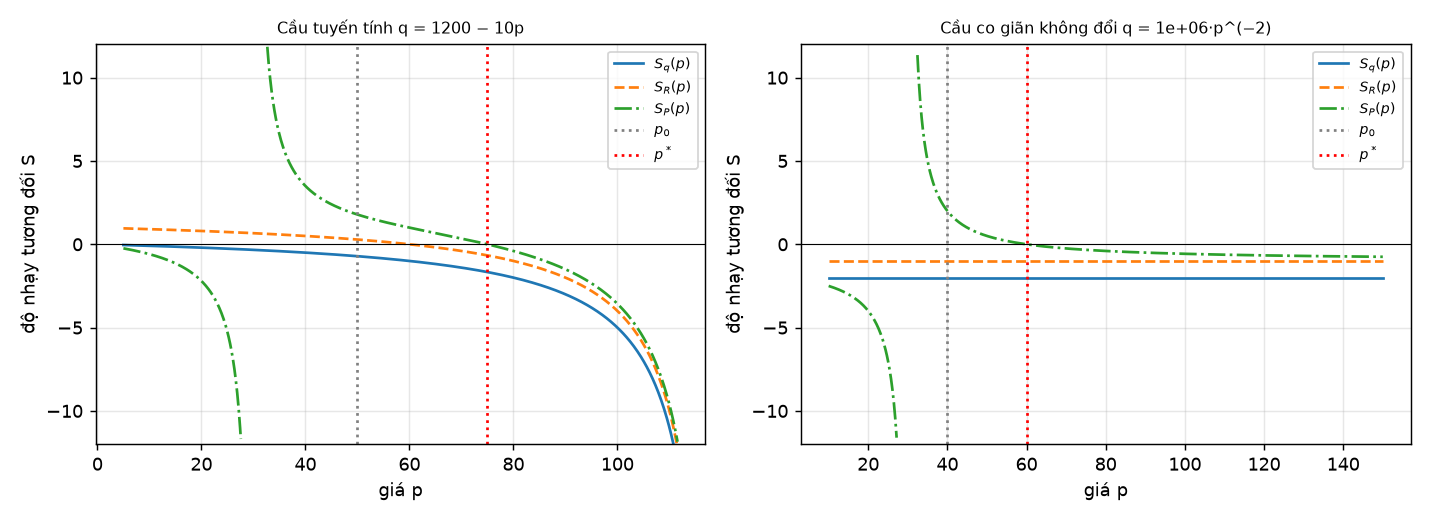
\includegraphics[width=\textwidth]{TN4_elasticity.png}
\caption{Độ nhạy $S_q$, $S_R$, $S_P$ theo giá $p$ (đường chấm: $p_0$ và $p^*$).}\label{fig:tn4}
\end{figure}

\subsection{TN5: Ảnh hưởng của tham số mô hình}
Cố định $\Delta p=+10\%$ và thay đổi độ dốc cầu $b$ (mô hình L) hoặc độ co giãn $k$ (mô hình E); các
bảng cho $E_{\mathrm{rel}}$ của $q$, $R$, $P$.

\begin{center}
\linespread{1}\small\selectfont
\begin{minipage}[t]{0.48\textwidth}\centering
\captionof{table}{Mô hình (L): $E_{\mathrm{rel}}$ (\%) khi thay đổi $b$.}\label{tab:tn5l}
% Tự sinh bởi make_tables.py - không sửa tay.

\begin{tabular}{@{}rrrr@{}}
\toprule
$b$ & $q$ & $R$ & $P$ \\
\midrule
$5{,}0$ & $0{,}0$ & $3{,}7$ & $3{,}0$ \\
$7{,}5$ & $0{,}0$ & $9{,}1$ & $5{,}9$ \\
$10{,}0$ & $0{,}0$ & $33{,}3$ & $11{,}1$ \\
$12{,}5$ & $0{,}0$ & $55{,}6$ & $23{,}8$ \\
$15{,}0$ & $0{,}0$ & $20{,}0$ & $100{,}0$ \\
$17{,}5$ & $0{,}0$ & $13{,}7$ & $77{,}8$ \\
$20{,}0$ & $0{,}0$ & $11{,}1$ & $33{,}3$ \\
\bottomrule
\end{tabular}

\end{minipage}\hfill
\begin{minipage}[t]{0.48\textwidth}\centering
\captionof{table}{Mô hình (E): $E_{\mathrm{rel}}$ (\%) khi thay đổi $k$.}\label{tab:tn5e}
% Tự sinh bởi make_tables.py - không sửa tay.

\begin{tabular}{@{}rrrr@{}}
\toprule
$k$ & $q$ & $R$ & $P$ \\
\midrule
$1{,}2$ & $11{,}0$ & $5{,}9$ & $12{,}6$ \\
$1{,}5$ & $12{,}6$ & $7{,}4$ & $17{,}1$ \\
$2{,}0$ & $15{,}2$ & $10{,}0$ & $27{,}4$ \\
$2{,}5$ & $17{,}9$ & $12{,}6$ & $45{,}4$ \\
$3{,}0$ & $20{,}6$ & $15{,}2$ & $92{,}9$ \\
$4{,}0$ & $26{,}2$ & $20{,}6$ & $100{,}0$ \\
\bottomrule
\end{tabular}

\end{minipage}
\end{center}

\begin{figure}[ht]
\centering
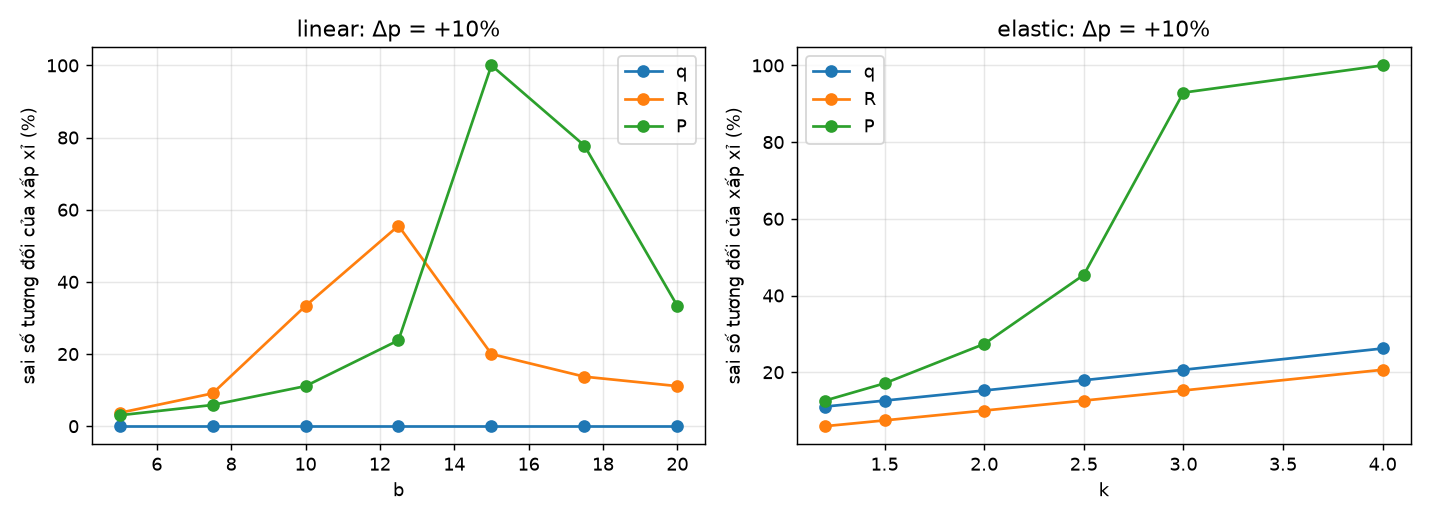
\includegraphics[width=\textwidth]{TN5_param_study.png}
\caption{Sai số tương đối của xấp xỉ vi phân khi $\Delta p=+10\%$ theo tham số mô hình.}\label{fig:tn5}
\end{figure}

Ở (L), $q$ luôn có sai số $0$. Sai số của $P$ không đơn điệu theo $b$: nó đạt $100\%$ tại $b=15$, vì khi
đó $p^*=(a+bc)/(2b)=55$ đúng bằng giá mới $p_0+10\%$, nên $\Delta P=dP/2$. Sai số của $R$ lớn nhất ở
$b=12{,}5$, gần $b=12$ là lúc $R'(p_0)=a-2bp_0=0$. Ở (E), sai số của cả ba đại lượng tăng theo $k$;
$P$ đạt $100\%$ tại $k=4$ vì khi đó $p^*=ck/(k-1)=40=p_0$, tức $P'(p_0)=0$ và $dP=0$.

\subsection{TN6: Mô phỏng Monte Carlo}
Giá thực tế $p=p_0(1+\varepsilon)$, $\varepsilon\sim N(0,\sigma^2)$, $N=200\,000$ mẫu, hạt giống
$20260503$. Bảng~\ref{tab:tn6} so sánh trung bình và độ lệch chuẩn của $\Delta P$ với
dự đoán~\eqref{eq:mc} (đơn vị nghìn đồng/tuần); Hình~\ref{fig:tn6} là phân bố của $\Delta P$ ở mô hình (L)
với $\sigma=10\%$.

\begin{table}[ht]
\tbsty
\caption{Monte Carlo: $\Delta P$ thực và dự đoán từ khai triển Taylor.}\label{tab:tn6}
{\setlength{\tabcolsep}{5pt}% Tự sinh bởi make_tables.py - không sửa tay.

\begin{tabular}{@{}llcrrrr@{}}
\toprule
Mô hình & Điểm & $\sigma$ (\%) & std thực & std dự đoán & mean thực & mean dự đoán \\
\midrule
Tuyến tính (L) & $p_0$ & $1$ & $248{,}50$ & $250{,}00$ & ${-}3{,}36$ & ${-}2{,}50$ \\
 & $p_0$ & $5$ & $1\,245{,}70$ & $1\,250{,}00$ & ${-}66{,}17$ & ${-}62{,}50$ \\
 & $p_0$ & $10$ & $2\,510{,}27$ & $2\,500{,}00$ & ${-}255{,}82$ & ${-}250{,}00$ \\
 & $p^*$ & $1$ & $7{,}85$ & $0{,}00$ & ${-}5{,}56$ & ${-}5{,}62$ \\
 & $p^*$ & $5$ & $196{,}22$ & $0{,}00$ & ${-}138{,}91$ & ${-}140{,}62$ \\
 & $p^*$ & $10$ & $784{,}86$ & $0{,}00$ & ${-}555{,}63$ & ${-}562{,}50$ \\
\midrule
Co giãn (E) & $p_0$ & $1$ & $124{,}47$ & $125{,}00$ & ${-}3{,}53$ & ${-}3{,}12$ \\
 & $p_0$ & $5$ & $650{,}40$ & $625{,}00$ & ${-}80{,}72$ & ${-}78{,}12$ \\
 & $p_0$ & $10$ & $1\,499{,}47$ & $1\,250{,}00$ & ${-}335{,}37$ & ${-}312{,}50$ \\
 & $p^*$ & $1$ & $1{,}17$ & $0{,}00$ & ${-}0{,}82$ & ${-}0{,}83$ \\
 & $p^*$ & $5$ & $31{,}55$ & $0{,}00$ & ${-}21{,}06$ & ${-}20{,}83$ \\
 & $p^*$ & $10$ & $159{,}18$ & $0{,}00$ & ${-}90{,}44$ & ${-}83{,}33$ \\
\bottomrule
\end{tabular}
}
\end{table}

Tại $p_0$, độ lệch chuẩn mô phỏng sát dự đoán $|P'|p_0\sigma$ (ví dụ $248{,}5$ so với $250{,}0$ ở (L),
$\sigma=1\%$), và trung bình âm sát $\tfrac12P''(p_0\sigma)^2$; độ lệch tăng khi $\sigma$ lớn ở mô
hình (E) ($1\,499$ so với $1\,250$ khi $\sigma=10\%$). Tại $p^*$ dự đoán bậc nhất của độ lệch chuẩn
bằng $0$ nhưng mô phỏng cho giá trị dương và trung bình âm, phù hợp với $\Delta P\approx\tfrac12P''(p^*\varepsilon)^2\le0$:
với $\sigma=5\%$, công thức $|P''|(p^*\sigma)^2/\sqrt2$ cho $198{,}9$ (L) và $29{,}5$ (E), so với $196{,}2$ và
$31{,}5$ mô phỏng.

\begin{figure}[ht]
\centering
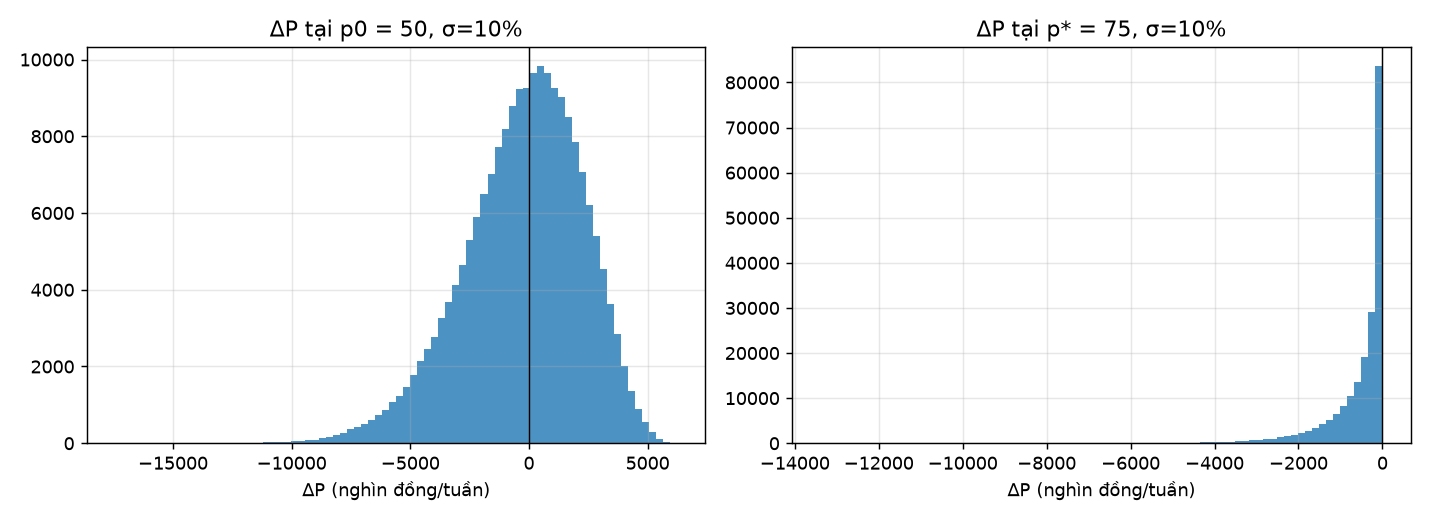
\includegraphics[width=\textwidth]{TN6_montecarlo_hist.png}
\caption{Phân bố của $\Delta P$ ở mô hình (L), $\sigma=10\%$: tại $p_0$ (trái) và tại $p^*$ (phải).}\label{fig:tn6}
\end{figure}

\subsection{TN7: Vùng tin cậy của vi phân}
Bảng~\ref{tab:tn7} cho mức lệch giá lớn nhất (tính theo $\%$ của $p_0$, dạng ``tăng\,/\,giảm'') để
$E_{\mathrm{rel}}\le\tau$; ``$\geq 50$'' nghĩa là không chạm ngưỡng trong khoảng khảo sát.

\begin{table}[ht]
\tbsty
\caption{Vùng tin cậy của vi phân (đơn vị: $\%$ của $p_0$).}\label{tab:tn7}
% Tự sinh bởi make_tables.py - không sửa tay.

\begin{tabular}{@{}llcccc@{}}
\toprule
Mô hình & Đại lượng & Điểm & $\tau=1\%$ & $\tau=5\%$ & $\tau=10\%$ \\
\midrule
Tuyến tính (L) & $q$ & $p_0$ & $\geq 50$ & $\geq 50$ & $\geq 50$ \\
 & $R$ & $p_0$ & ${+}0{,}35\,/\,{-}0{,}40$ & ${+}1{,}90\,/\,{-}2{,}10$ & ${+}3{,}60\,/\,{-}4{,}40$ \\
 & $P$ & $p_0$ & ${+}0{,}95\,/\,{-}1{,}00$ & ${+}4{,}75\,/\,{-}5{,}25$ & ${+}9{,}05\,/\,{-}11{,}10$ \\
 & $P$ & $p^*$ & ${+}0{,}00\,/\,{-}0{,}00$ & ${+}0{,}00\,/\,{-}0{,}00$ & ${+}0{,}00\,/\,{-}0{,}00$ \\
\midrule
Co giãn (E) & $q$ & $p_0$ & ${+}0{,}65\,/\,{-}0{,}65$ & ${+}3{,}30\,/\,{-}3{,}35$ & ${+}6{,}55\,/\,{-}6{,}70$ \\
 & $R$ & $p_0$ & ${+}0{,}95\,/\,{-}1{,}00$ & ${+}5{,}00\,/\,{-}5{,}00$ & ${+}9{,}95\,/\,{-}10{,}00$ \\
 & $P$ & $p_0$ & ${+}0{,}35\,/\,{-}0{,}40$ & ${+}1{,}95\,/\,{-}2{,}00$ & ${+}3{,}85\,/\,{-}4{,}15$ \\
 & $P$ & $p^*$ & ${+}0{,}00\,/\,{-}0{,}00$ & ${+}0{,}00\,/\,{-}0{,}00$ & ${+}0{,}00\,/\,{-}0{,}00$ \\
\bottomrule
\end{tabular}

\end{table}

Vùng tin cậy tăng xấp xỉ tỉ lệ với $\tau$ (ví dụ $P$ ở (L): $0{,}95$; $4{,}75$; $9{,}05$ cho $\tau=1;5;10\%$),
đúng như ước lượng~\eqref{eq:safe}. Với cùng $\tau=5\%$, ở (L) $R$ có vùng hẹp nhất ($+1{,}90/-2{,}10$)
còn $q$ chính xác tuyệt đối, trong khi ở (E) $P$ hẹp nhất ($+1{,}95/-2{,}00$). Tại $p^*$ vùng bằng $0$.

\begin{figure}[ht]
\centering
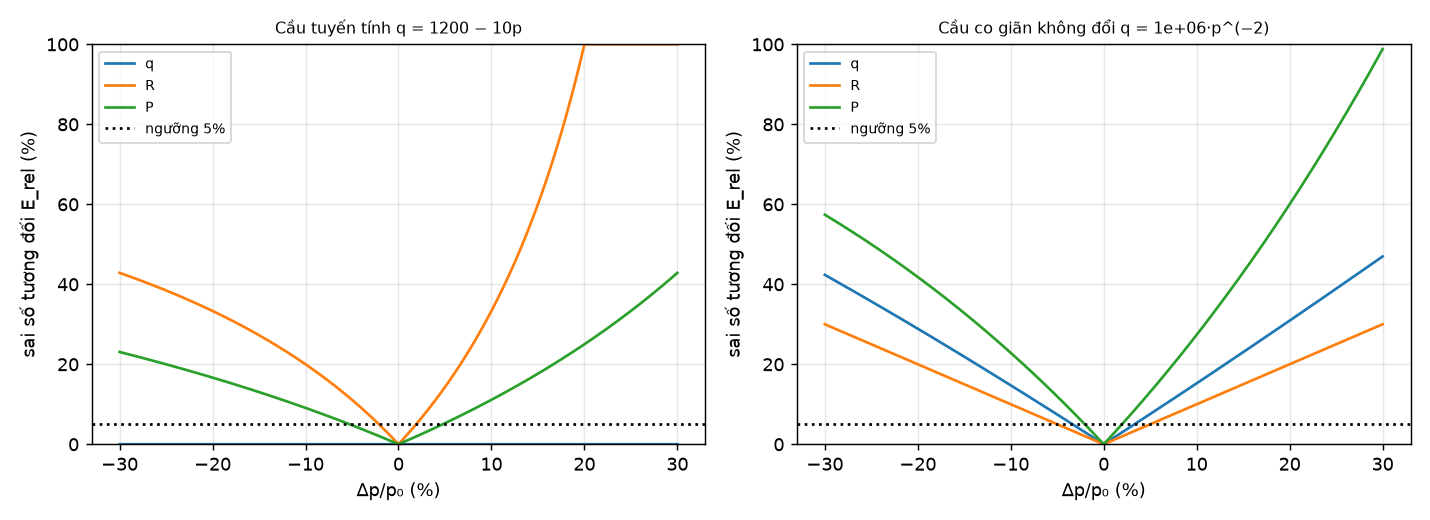
\includegraphics[width=\textwidth]{TN7_erel_vs_delta.png}
\caption{$E_{\mathrm{rel}}$ theo $\Delta p/p_0$ tại $p_0$ (đường chấm: ngưỡng $5\%$).}\label{fig:tn7}
\end{figure}

\subsection{TN8: Xấp xỉ bậc hai}
Bảng~\ref{tab:tn8} so sánh vi phân bậc một $dP$ và xấp xỉ bậc hai $dP_2$ cho $P$ ở mô hình (E).
Ở mô hình (L), $R$ và $P$ là đa thức bậc hai nên $dP_2$ trùng $\Delta P$ ở mọi dòng (sai số $0$).

\begin{table}[ht]
\tbsty
\caption{Mô hình (E): $P$ tại $p_0=40$ và $p^*=60$, xấp xỉ bậc một và bậc hai.}\label{tab:tn8}
{\setlength{\tabcolsep}{5pt}% Tự sinh bởi make_tables.py - không sửa tay.

\begin{tabular}{@{}clrrrrr@{}}
\toprule
Điểm & $\Delta p/p_0$ (\%) & $\Delta P$ thực & $dP$ (bậc 1) & $dP_2$ (bậc 2) & $E_{\mathrm{rel}}$ bậc 1 (\%) & $E_{\mathrm{rel}}$ bậc 2 (\%) \\
\midrule
$p_0$ & ${-}20$ & ${-}4\,296{,}9$ & ${-}2\,500{,}0$ & ${-}3\,750{,}0$ & $41{,}82$ & $12{,}73$ \\
 & ${-}10$ & ${-}1\,620{,}4$ & ${-}1\,250{,}0$ & ${-}1\,562{,}5$ & $22{,}86$ & $3{,}57$ \\
 & ${-}5$ & ${-}709{,}8$ & ${-}625{,}0$ & ${-}703{,}1$ & $11{,}95$ & $0{,}95$ \\
 & ${+}5$ & $552{,}7$ & $625{,}0$ & $546{,}9$ & $13{,}08$ & $1{,}06$ \\
 & ${+}10$ & $981{,}4$ & $1\,250{,}0$ & $937{,}5$ & $27{,}37$ & $4{,}47$ \\
 & ${+}20$ & $1\,562{,}5$ & $2\,500{,}0$ & $1\,250{,}0$ & $60{,}00$ & $20{,}00$ \\
\midrule
$p^*$ & ${-}20$ & ${-}520{,}8$ & $0{,}0$ & ${-}333{,}3$ & $100{,}00$ & $36{,}00$ \\
 & ${-}10$ & ${-}102{,}9$ & $0{,}0$ & ${-}83{,}3$ & $100{,}00$ & $19{,}00$ \\
 & ${-}5$ & ${-}23{,}1$ & $0{,}0$ & ${-}20{,}8$ & $100{,}00$ & $9{,}75$ \\
 & ${+}5$ & ${-}18{,}9$ & $0{,}0$ & ${-}20{,}8$ & $100{,}00$ & $10{,}25$ \\
 & ${+}10$ & ${-}68{,}9$ & $0{,}0$ & ${-}83{,}3$ & $100{,}00$ & $21{,}00$ \\
 & ${+}20$ & ${-}231{,}5$ & $0{,}0$ & ${-}333{,}3$ & $100{,}00$ & $44{,}00$ \\
\bottomrule
\end{tabular}
}
\end{table}

Tại $p_0$ với $\Delta p/p_0=+5\%$, $E_{\mathrm{rel}}$ giảm từ $13{,}08\%$ xuống $1{,}06\%$; với $+10\%$ từ
$27{,}37\%$ xuống $4{,}47\%$; với $+20\%$ từ $60{,}00\%$ xuống $20{,}00\%$. Tại $p^*$, vi phân bậc một cho
$dP=0$ ($E_{\mathrm{rel}}=100\%$) còn $dP_2$ bắt được thay đổi thực với sai số $10{,}25\%$ ($+5\%$) và
$9{,}75\%$ ($-5\%$). Hệ số góc log-log (Bảng~\ref{tab:tn8o}, Hình~\ref{fig:tn8}) xấp xỉ $2$ cho bậc một và
xấp xỉ $3$ cho bậc hai ($2{,}95$ đến $2{,}96$ ở mô hình E), khớp với lý thuyết ở Mục~\ref{sec:phuongphap}.

\begin{table}[ht]
\tbsty
\caption{Hệ số góc log-log của sai số xấp xỉ bậc một và bậc hai. Dấu ``---'': sai số bằng $0$.}\label{tab:tn8o}
% Tự sinh bởi make_tables.py - không sửa tay.

\begin{tabular}{@{}llcrr@{}}
\toprule
Mô hình & Đại lượng & Điểm & Bậc 1 & Bậc 2 \\
\midrule
Tuyến tính (L) & $R$ & $p_0$ & $2{,}000$ & --- \\
 & $P$ & $p_0$ & $2{,}000$ & --- \\
 & $P$ & $p^*$ & $2{,}000$ & --- \\
\midrule
Co giãn (E) & $R$ & $p_0$ & $1{,}980$ & $2{,}964$ \\
 & $P$ & $p_0$ & $1{,}968$ & $2{,}960$ \\
 & $P$ & $p^*$ & $1{,}959$ & $2{,}950$ \\
\bottomrule
\end{tabular}

\end{table}

\begin{figure}[ht]
\centering
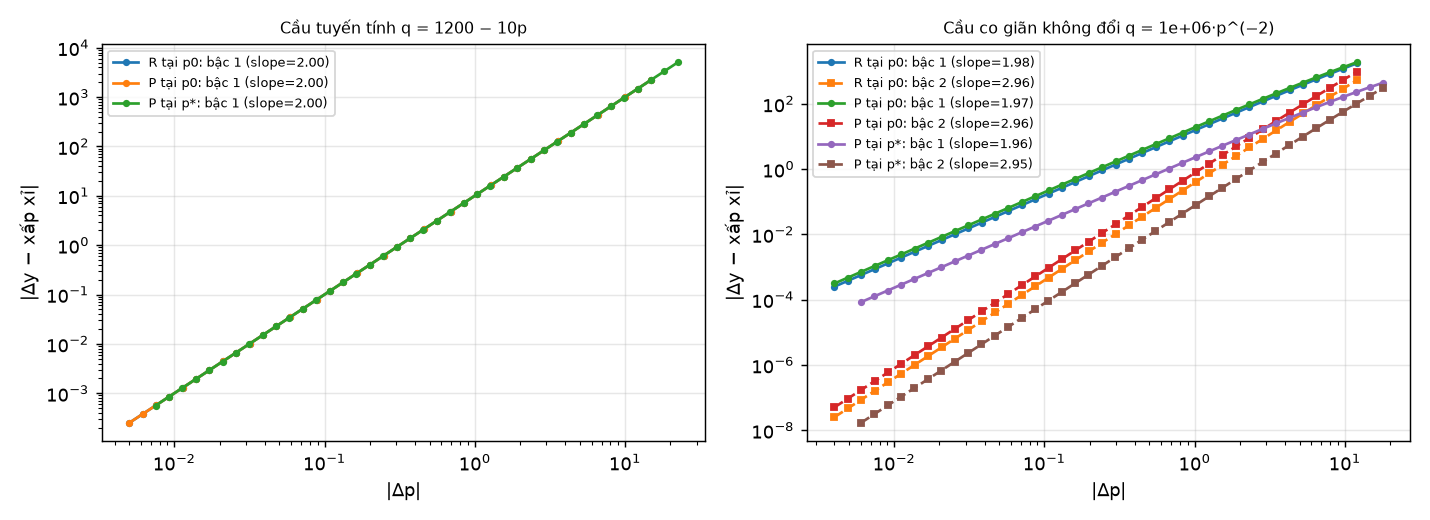
\includegraphics[width=\textwidth]{TN8_second_order_loglog.png}
\caption{Sai số của xấp xỉ bậc một và bậc hai theo $|\Delta p|$ (log-log).}\label{fig:tn8}
\end{figure}
.
% Cần: amsmath, booktabs, graphicx. Bảng nằm trong generated/ (tự sinh bởi
% make_tables.py từ output/tables), hình nằm trong ../output/figures.
% Chỉ nêu SỐ LIỆU quan sát được; phần diễn giải ý nghĩa thuộc Mục kết quả và phân tích.
% ============================================================
\section{Tính toán, mô phỏng và thực nghiệm}\label{sec:thucnghiem}

\subsection{Cài đặt và kiểm chứng}
Chương trình được viết bằng Python (NumPy, pandas, Matplotlib) và chia thành các tệp
riêng: \texttt{src/model.py} (hai mô hình cầu và các đạo hàm tính tay),
\texttt{src/sensitivity.py} (thay đổi thực, vi phân, sai số, độ nhạy, bậc hội tụ, xấp xỉ
bậc hai, vùng tin cậy), \texttt{src/montecarlo.py} (mô phỏng nhiễu giá),
\texttt{experiments.py} (chạy các thí nghiệm, xuất bảng CSV và hình PNG) và
\texttt{app.py} (ứng dụng tương tác dùng chung mã với báo cáo). Phần mềm chỉ dùng để
tính toán, vẽ đồ thị và kiểm chứng: mọi đạo hàm và công thức sai số được cài đặt từ
các biểu thức ở Mục~\ref{sec:phuongphap}, không gọi hàm có sẵn để tạo kết quả chính.

Việc kiểm chứng do \texttt{verify.py} thực hiện: với $40$ điểm trong miền xác định, các hàm
$q,R,P$ và đạo hàm cấp một, cấp hai cài đặt trong chương trình khớp SymPy với sai lệch
tương đối nhỏ hơn $10^{-9}$, và đạo hàm cấp một khớp sai phân trung tâm với sai lệch
tương đối nhỏ hơn $10^{-5}$; ngoài ra $P'(p^*)=0$ với sai số dưới $10^{-8}$.
Mọi số liệu dưới đây được sinh lại bằng một lệnh (\texttt{uv run experiments.py}) với hạt
giống mô phỏng cố định, nên chạy lại cho kết quả giống hệt.

Tám thí nghiệm (TN) được thực hiện trên hai mô hình ở Bảng~\ref{tab:par}:

\begin{table}[ht]
\tbsty
\caption{Các thí nghiệm và công cụ Giải tích tương ứng.}\label{tab:tn}
\begin{tabular}{@{}l p{6.2cm} p{6.2cm}@{}}
\toprule
TN & Câu hỏi & Công cụ \\
\midrule
1 & Vi phân dự báo thay đổi thực tốt đến đâu? & vi phân, sai số tuyệt đối/tương đối \\
2 & Xấp xỉ tuyến tính trông thế nào? & tiếp tuyến \\
3 & Sai số giảm theo $\Delta p$ với bậc bao nhiêu? & khai triển Taylor, hồi quy log-log \\
4 & Đại lượng nào nhạy nhất với giá? & độ nhạy tương đối $S$ \\
5 & Kết quả có đổi khi đổi tham số mô hình không? & quét $b$ (L) và $k$ (E) \\
6 & Giá nhiễu ngẫu nhiên thì $\Delta P$ phân bố ra sao? & Monte Carlo, Taylor \\
7 & Vi phân dùng được đến mức lệch giá nào? & vùng tin cậy theo ngưỡng $\tau$ \\
8 & Thêm số hạng bậc hai cải thiện bao nhiêu? & xấp xỉ Taylor bậc hai \\
\bottomrule
\end{tabular}
\end{table}

\subsection{TN1: So sánh thay đổi thực và vi phân}
Với mỗi mức lệch $\Delta p/p_0\in\{\pm1,\pm2,\pm5,\pm10,\pm20\}\%$ ta tính $\Delta P$ thực,
$dP=P'(p_0)\Delta p$ và sai số (Bảng~\ref{tab:tn1l} và~\ref{tab:tn1e}; đơn vị của $\Delta P$,
$dP$ là nghìn đồng/tuần).

\begin{table}[ht]
\tbsty
\caption{Lợi nhuận $P$ tại $p_0=50$, mô hình (L).}\label{tab:tn1l}
% Tự sinh bởi make_tables.py - không sửa tay.

\begin{tabular}{@{}rrrrr@{}}
\toprule
$\Delta p/p_0$ (\%) & $\Delta P$ thực & $dP$ & $|\Delta P-dP|$ & $E_{\mathrm{rel}}$ (\%) \\
\midrule
${-}20$ & ${-}6\,000{,}0$ & ${-}5\,000{,}0$ & $1\,000{,}0$ & $16{,}67$ \\
${-}10$ & ${-}2\,750{,}0$ & ${-}2\,500{,}0$ & $250{,}0$ & $9{,}09$ \\
${-}5$ & ${-}1\,312{,}5$ & ${-}1\,250{,}0$ & $62{,}5$ & $4{,}76$ \\
${-}2$ & ${-}510{,}0$ & ${-}500{,}0$ & $10{,}0$ & $1{,}96$ \\
${-}1$ & ${-}252{,}5$ & ${-}250{,}0$ & $2{,}5$ & $0{,}99$ \\
${+}1$ & $247{,}5$ & $250{,}0$ & $2{,}5$ & $1{,}01$ \\
${+}2$ & $490{,}0$ & $500{,}0$ & $10{,}0$ & $2{,}04$ \\
${+}5$ & $1\,187{,}5$ & $1\,250{,}0$ & $62{,}5$ & $5{,}26$ \\
${+}10$ & $2\,250{,}0$ & $2\,500{,}0$ & $250{,}0$ & $11{,}11$ \\
${+}20$ & $4\,000{,}0$ & $5\,000{,}0$ & $1\,000{,}0$ & $25{,}00$ \\
\bottomrule
\end{tabular}

\end{table}

\begin{table}[ht]
\tbsty
\caption{Lợi nhuận $P$ tại $p_0=40$, mô hình (E).}\label{tab:tn1e}
% Tự sinh bởi make_tables.py - không sửa tay.

\begin{tabular}{@{}rrrrr@{}}
\toprule
$\Delta p/p_0$ (\%) & $\Delta P$ thực & $dP$ & $|\Delta P-dP|$ & $E_{\mathrm{rel}}$ (\%) \\
\midrule
${-}20$ & ${-}4\,296{,}9$ & ${-}2\,500{,}0$ & $1\,796{,}9$ & $41{,}82$ \\
${-}10$ & ${-}1\,620{,}4$ & ${-}1\,250{,}0$ & $370{,}4$ & $22{,}86$ \\
${-}5$ & ${-}709{,}8$ & ${-}625{,}0$ & $84{,}8$ & $11{,}95$ \\
${-}2$ & ${-}262{,}9$ & ${-}250{,}0$ & $12{,}9$ & $4{,}91$ \\
${-}1$ & ${-}128{,}2$ & ${-}125{,}0$ & $3{,}2$ & $2{,}48$ \\
${+}1$ & $121{,}9$ & $125{,}0$ & $3{,}1$ & $2{,}52$ \\
${+}2$ & $237{,}9$ & $250{,}0$ & $12{,}1$ & $5{,}09$ \\
${+}5$ & $552{,}7$ & $625{,}0$ & $72{,}3$ & $13{,}08$ \\
${+}10$ & $981{,}4$ & $1\,250{,}0$ & $268{,}6$ & $27{,}37$ \\
${+}20$ & $1\,562{,}5$ & $2\,500{,}0$ & $937{,}5$ & $60{,}00$ \\
\bottomrule
\end{tabular}

\end{table}

Ở mô hình (L), $E_{\mathrm{rel}}$ tăng từ $1{,}0\%$ ($\Delta p/p_0=\pm1\%$) lên $5{,}3\%$
($+5\%$) và $25{,}0\%$ ($+20\%$); ở mô hình (E) từ $2{,}5\%$ lên $13{,}1\%$ và $60{,}0\%$. Với
(L), $P$ là hàm bậc hai nên $|\Delta P-dP|=\tfrac12|P''|\Delta p^2$ đối xứng giữa hai phía
(ví dụ $62{,}5$ cho cả $\pm5\%$), còn $E_{\mathrm{rel}}$ không đối xứng ($4{,}76\%$ và $5{,}26\%$)
vì $\Delta P$ ở hai phía khác nhau.

Tại giá tối ưu $p^*$ (với $P'(p^*)=0$) thì $dP=0$; thay đổi thực khi giá tăng $5\%$ là
$-140{,}6$ (mô hình L, $p^*=75$) và $-18{,}9$ (mô hình E, $p^*=60$), nên $E_{\mathrm{rel}}=100\%$.
Với $q$ và $R$, kết quả tương tự được lưu trong \texttt{output/tables/}.

\subsection{TN2: Tiếp tuyến và đường cong}
Hình~\ref{fig:tn2l} và~\ref{fig:tn2e} vẽ $q,R,P$ cùng tiếp tuyến tại $p_0$; dải tô màu là
$p_0\pm20\%$. Khoảng cách giữa đường cong và tiếp tuyến chính là sai số của xấp xỉ vi phân,
nhỏ gần $p_0$ và tăng nhanh khi ra xa.

\begin{figure}[ht]
\centering
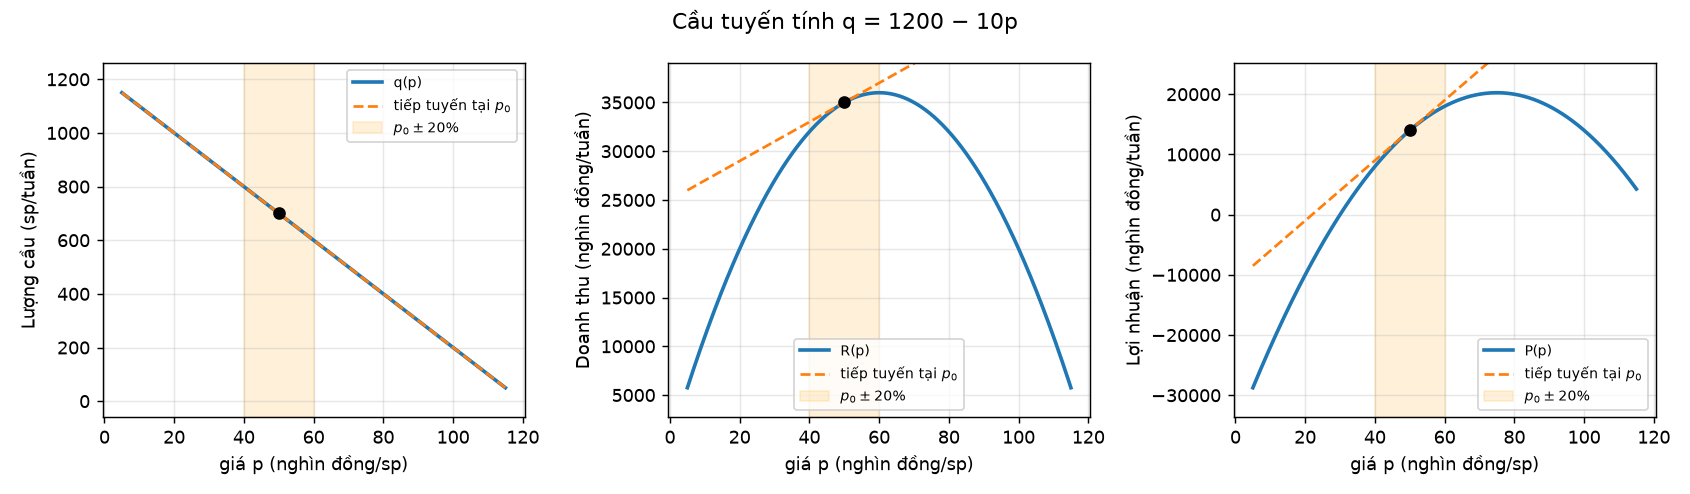
\includegraphics[width=\textwidth]{TN2_tangent_linear.png}
\caption{Mô hình (L): $q$, $R$, $P$ và tiếp tuyến tại $p_0=50$.}\label{fig:tn2l}
\end{figure}
\begin{figure}[ht]
\centering
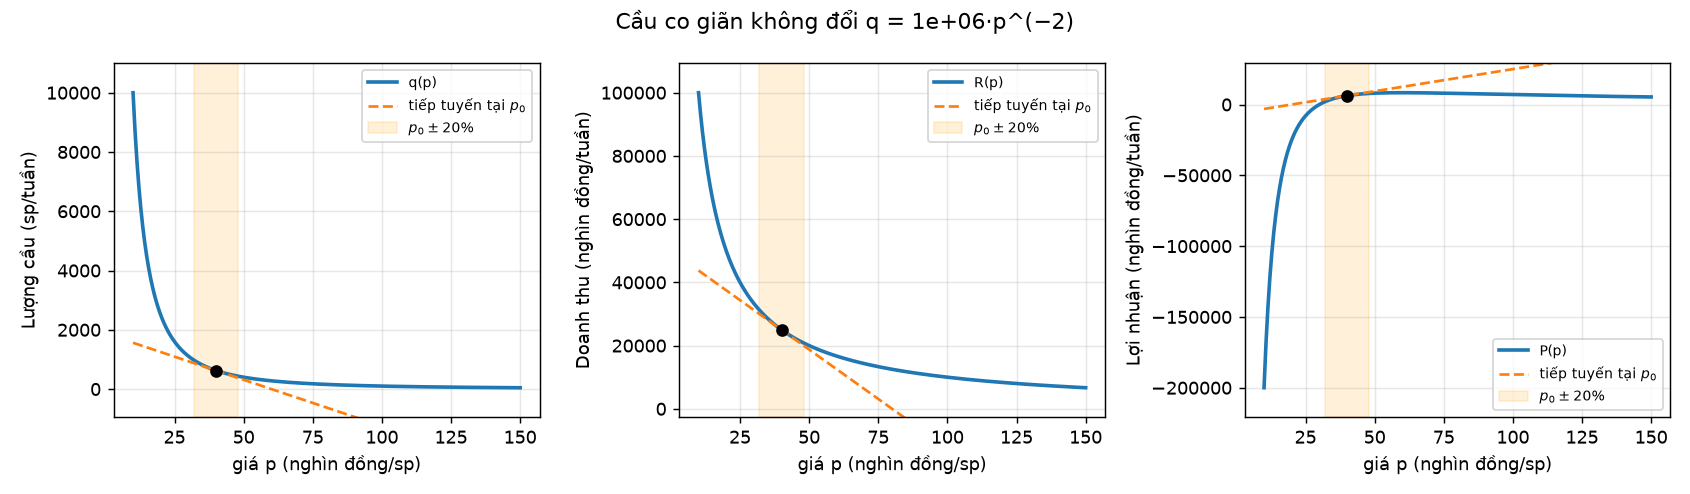
\includegraphics[width=\textwidth]{TN2_tangent_elastic.png}
\caption{Mô hình (E): $q$, $R$, $P$ và tiếp tuyến tại $p_0=40$.}\label{fig:tn2e}
\end{figure}

\subsection{TN3: Bậc của sai số}
Hệ số góc log-log của $E_{\mathrm{abs}}$ theo $|\Delta p|$ (cách đo ở Mục~\ref{sec:phuongphap}) cho trong
Bảng~\ref{tab:tn3}; kỳ vọng là $2$.

\begin{table}[ht]
\tbsty
\caption{Hệ số góc log-log của sai số vi phân. Dấu ``---'': sai số bằng $0$.}\label{tab:tn3}
% Tự sinh bởi make_tables.py - không sửa tay.

\begin{tabular}{@{}llcr@{}}
\toprule
Mô hình & Đại lượng & Điểm & Hệ số góc log-log \\
\midrule
Tuyến tính (L) & $q$ & $p_0$ & --- \\
 & $R$ & $p_0$ & $2{,}000$ \\
 & $P$ & $p_0$ & $2{,}000$ \\
 & $P$ & $p^*$ & $2{,}000$ \\
\midrule
Co giãn (E) & $q$ & $p_0$ & $1{,}973$ \\
 & $R$ & $p_0$ & $1{,}980$ \\
 & $P$ & $p_0$ & $1{,}968$ \\
 & $P$ & $p^*$ & $1{,}959$ \\
\bottomrule
\end{tabular}

\end{table}

Ở (L), $R$ và $P$ cho đúng $2{,}000$, còn $q$ là hàm tuyến tính nên sai số bằng $0$. Ở (E), các
hệ số góc nằm trong khoảng $1{,}96$ đến $1{,}98$, gần $2$ nhưng hơi lệch vì lưới $\Delta p$ trải đến
$30\%$ nên các số hạng bậc cao bắt đầu có ảnh hưởng (Hình~\ref{fig:tn3}).

\begin{figure}[ht]
\centering
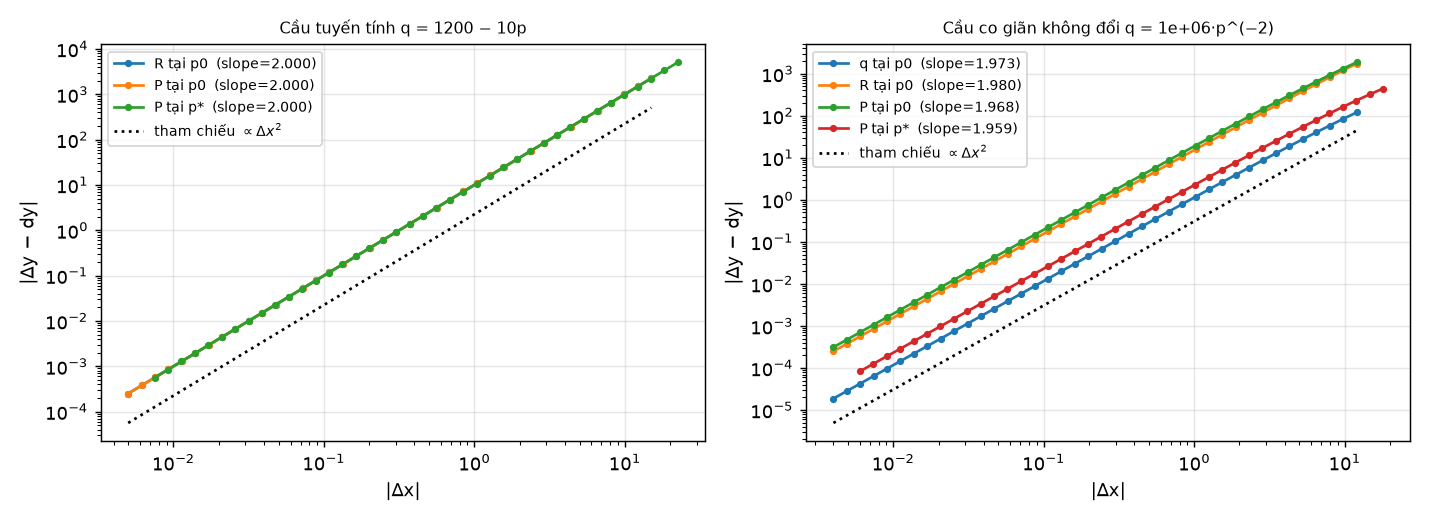
\includegraphics[width=\textwidth]{TN3_error_loglog.png}
\caption{Sai số $|\Delta y-dy|$ theo $|\Delta p|$ (thang log-log) và đường tham chiếu $\propto\Delta p^2$.}\label{fig:tn3}
\end{figure}

\subsection{TN4: Độ nhạy tương đối}
Bảng~\ref{tab:tn4} cho $S=f'p/f$ tại $p_0$ và $p^*$; Hình~\ref{fig:tn4} vẽ $S(p)$ (cắt ở $|S|>12$).

\begin{table}[ht]
\tbsty
\caption{Độ nhạy tương đối của $q$, $R$, $P$ theo giá.}\label{tab:tn4}
% Tự sinh bởi make_tables.py - không sửa tay.

\begin{tabular}{@{}llrr@{}}
\toprule
Mô hình & Độ nhạy & tại $p_0$ & tại $p^*$ \\
\midrule
Tuyến tính (L) & $S_q$ & ${-}0{,}714$ & ${-}1{,}667$ \\
 & $S_R$ & $0{,}286$ & ${-}0{,}667$ \\
 & $S_P$ & $1{,}786$ & $0{,}000$ \\
\midrule
Co giãn (E) & $S_q$ & ${-}2{,}000$ & ${-}2{,}000$ \\
 & $S_R$ & ${-}1{,}000$ & ${-}1{,}000$ \\
 & $S_P$ & $2{,}000$ & $0{,}000$ \\
\bottomrule
\end{tabular}

\end{table}

Tại $p_0$, ở (L) $|S_P|=1{,}786$ lớn nhất, sau đó là $|S_q|=0{,}714$ và $|S_R|=0{,}286$; ở (E)
$S_q=-2$, $S_R=-1$, $S_P=2$, trong đó $|S_P|$ và $|S_q|$ bằng nhau. Các giá trị khớp với hệ
thức~\eqref{eq:S}: ví dụ ở (L), $S_P=50/20-0{,}714=1{,}786$; ở (E), $S_P=40/10-2=2$. Tại $p^*$,
$S_P=0$ ở cả hai mô hình.

\begin{figure}[ht]
\centering
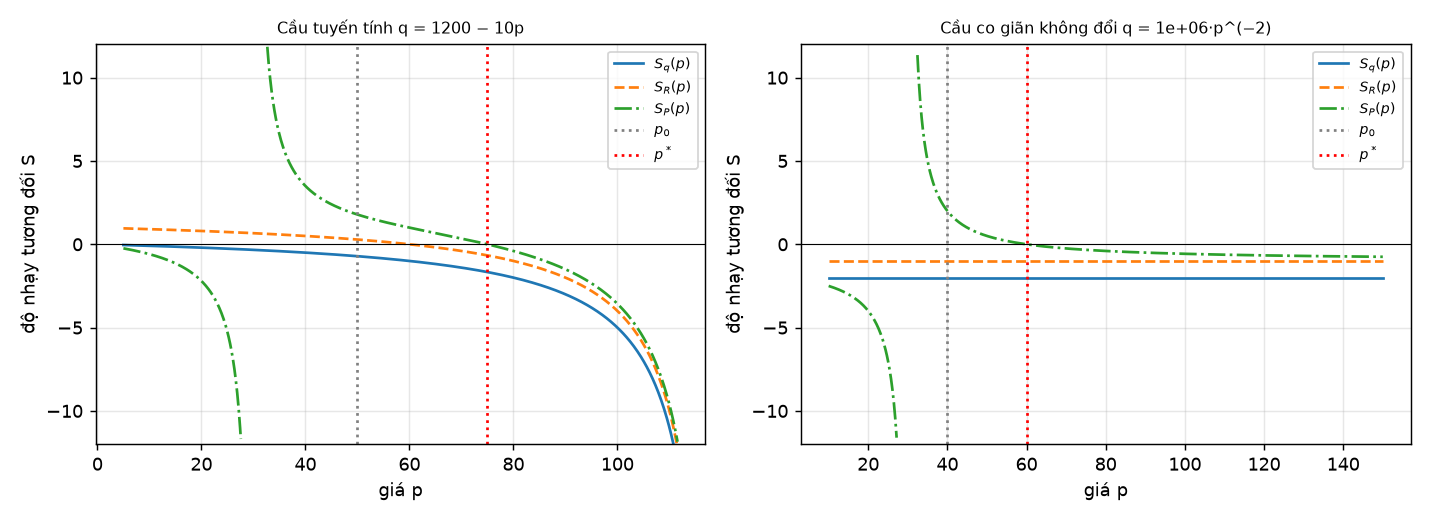
\includegraphics[width=\textwidth]{TN4_elasticity.png}
\caption{Độ nhạy $S_q$, $S_R$, $S_P$ theo giá $p$ (đường chấm: $p_0$ và $p^*$).}\label{fig:tn4}
\end{figure}

\subsection{TN5: Ảnh hưởng của tham số mô hình}
Cố định $\Delta p=+10\%$ và thay đổi độ dốc cầu $b$ (mô hình L) hoặc độ co giãn $k$ (mô hình E); các
bảng cho $E_{\mathrm{rel}}$ của $q$, $R$, $P$.

\begin{center}
\linespread{1}\small\selectfont
\begin{minipage}[t]{0.48\textwidth}\centering
\captionof{table}{Mô hình (L): $E_{\mathrm{rel}}$ (\%) khi thay đổi $b$.}\label{tab:tn5l}
% Tự sinh bởi make_tables.py - không sửa tay.

\begin{tabular}{@{}rrrr@{}}
\toprule
$b$ & $q$ & $R$ & $P$ \\
\midrule
$5{,}0$ & $0{,}0$ & $3{,}7$ & $3{,}0$ \\
$7{,}5$ & $0{,}0$ & $9{,}1$ & $5{,}9$ \\
$10{,}0$ & $0{,}0$ & $33{,}3$ & $11{,}1$ \\
$12{,}5$ & $0{,}0$ & $55{,}6$ & $23{,}8$ \\
$15{,}0$ & $0{,}0$ & $20{,}0$ & $100{,}0$ \\
$17{,}5$ & $0{,}0$ & $13{,}7$ & $77{,}8$ \\
$20{,}0$ & $0{,}0$ & $11{,}1$ & $33{,}3$ \\
\bottomrule
\end{tabular}

\end{minipage}\hfill
\begin{minipage}[t]{0.48\textwidth}\centering
\captionof{table}{Mô hình (E): $E_{\mathrm{rel}}$ (\%) khi thay đổi $k$.}\label{tab:tn5e}
% Tự sinh bởi make_tables.py - không sửa tay.

\begin{tabular}{@{}rrrr@{}}
\toprule
$k$ & $q$ & $R$ & $P$ \\
\midrule
$1{,}2$ & $11{,}0$ & $5{,}9$ & $12{,}6$ \\
$1{,}5$ & $12{,}6$ & $7{,}4$ & $17{,}1$ \\
$2{,}0$ & $15{,}2$ & $10{,}0$ & $27{,}4$ \\
$2{,}5$ & $17{,}9$ & $12{,}6$ & $45{,}4$ \\
$3{,}0$ & $20{,}6$ & $15{,}2$ & $92{,}9$ \\
$4{,}0$ & $26{,}2$ & $20{,}6$ & $100{,}0$ \\
\bottomrule
\end{tabular}

\end{minipage}
\end{center}

\begin{figure}[ht]
\centering
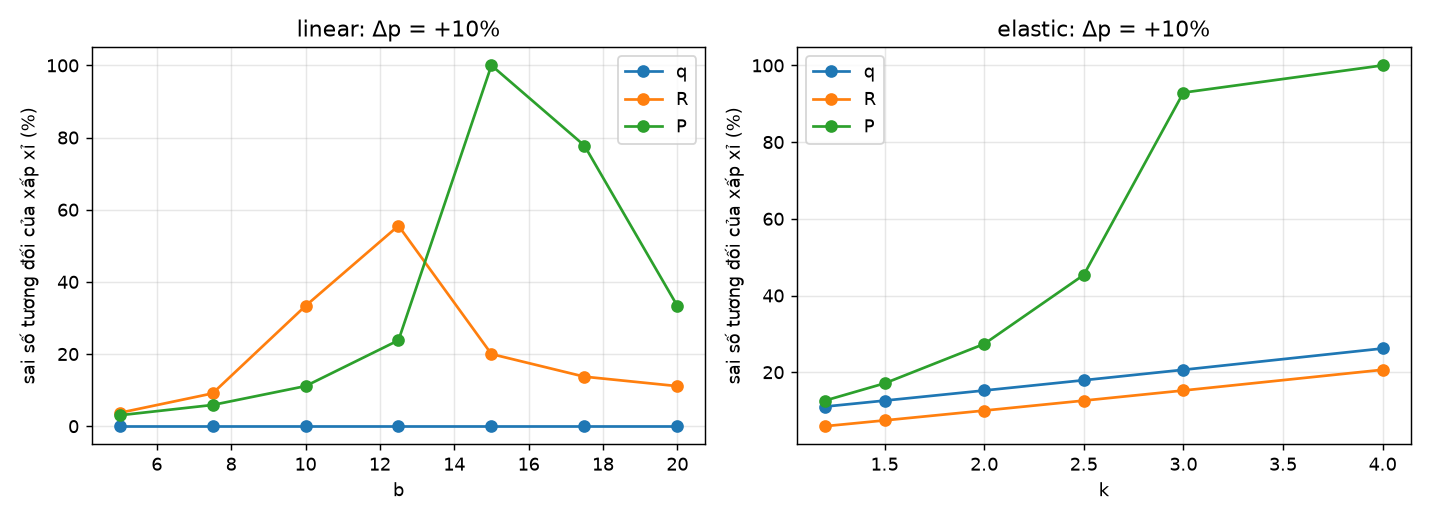
\includegraphics[width=\textwidth]{TN5_param_study.png}
\caption{Sai số tương đối của xấp xỉ vi phân khi $\Delta p=+10\%$ theo tham số mô hình.}\label{fig:tn5}
\end{figure}

Ở (L), $q$ luôn có sai số $0$. Sai số của $P$ không đơn điệu theo $b$: nó đạt $100\%$ tại $b=15$, vì khi
đó $p^*=(a+bc)/(2b)=55$ đúng bằng giá mới $p_0+10\%$, nên $\Delta P=dP/2$. Sai số của $R$ lớn nhất ở
$b=12{,}5$, gần $b=12$ là lúc $R'(p_0)=a-2bp_0=0$. Ở (E), sai số của cả ba đại lượng tăng theo $k$;
$P$ đạt $100\%$ tại $k=4$ vì khi đó $p^*=ck/(k-1)=40=p_0$, tức $P'(p_0)=0$ và $dP=0$.

\subsection{TN6: Mô phỏng Monte Carlo}
Giá thực tế $p=p_0(1+\varepsilon)$, $\varepsilon\sim N(0,\sigma^2)$, $N=200\,000$ mẫu, hạt giống
$20260503$. Bảng~\ref{tab:tn6} so sánh trung bình và độ lệch chuẩn của $\Delta P$ với
dự đoán~\eqref{eq:mc} (đơn vị nghìn đồng/tuần); Hình~\ref{fig:tn6} là phân bố của $\Delta P$ ở mô hình (L)
với $\sigma=10\%$.

\begin{table}[ht]
\tbsty
\caption{Monte Carlo: $\Delta P$ thực và dự đoán từ khai triển Taylor.}\label{tab:tn6}
{\setlength{\tabcolsep}{5pt}% Tự sinh bởi make_tables.py - không sửa tay.

\begin{tabular}{@{}llcrrrr@{}}
\toprule
Mô hình & Điểm & $\sigma$ (\%) & std thực & std dự đoán & mean thực & mean dự đoán \\
\midrule
Tuyến tính (L) & $p_0$ & $1$ & $248{,}50$ & $250{,}00$ & ${-}3{,}36$ & ${-}2{,}50$ \\
 & $p_0$ & $5$ & $1\,245{,}70$ & $1\,250{,}00$ & ${-}66{,}17$ & ${-}62{,}50$ \\
 & $p_0$ & $10$ & $2\,510{,}27$ & $2\,500{,}00$ & ${-}255{,}82$ & ${-}250{,}00$ \\
 & $p^*$ & $1$ & $7{,}85$ & $0{,}00$ & ${-}5{,}56$ & ${-}5{,}62$ \\
 & $p^*$ & $5$ & $196{,}22$ & $0{,}00$ & ${-}138{,}91$ & ${-}140{,}62$ \\
 & $p^*$ & $10$ & $784{,}86$ & $0{,}00$ & ${-}555{,}63$ & ${-}562{,}50$ \\
\midrule
Co giãn (E) & $p_0$ & $1$ & $124{,}47$ & $125{,}00$ & ${-}3{,}53$ & ${-}3{,}12$ \\
 & $p_0$ & $5$ & $650{,}40$ & $625{,}00$ & ${-}80{,}72$ & ${-}78{,}12$ \\
 & $p_0$ & $10$ & $1\,499{,}47$ & $1\,250{,}00$ & ${-}335{,}37$ & ${-}312{,}50$ \\
 & $p^*$ & $1$ & $1{,}17$ & $0{,}00$ & ${-}0{,}82$ & ${-}0{,}83$ \\
 & $p^*$ & $5$ & $31{,}55$ & $0{,}00$ & ${-}21{,}06$ & ${-}20{,}83$ \\
 & $p^*$ & $10$ & $159{,}18$ & $0{,}00$ & ${-}90{,}44$ & ${-}83{,}33$ \\
\bottomrule
\end{tabular}
}
\end{table}

Tại $p_0$, độ lệch chuẩn mô phỏng sát dự đoán $|P'|p_0\sigma$ (ví dụ $248{,}5$ so với $250{,}0$ ở (L),
$\sigma=1\%$), và trung bình âm sát $\tfrac12P''(p_0\sigma)^2$; độ lệch tăng khi $\sigma$ lớn ở mô
hình (E) ($1\,499$ so với $1\,250$ khi $\sigma=10\%$). Tại $p^*$ dự đoán bậc nhất của độ lệch chuẩn
bằng $0$ nhưng mô phỏng cho giá trị dương và trung bình âm, phù hợp với $\Delta P\approx\tfrac12P''(p^*\varepsilon)^2\le0$:
với $\sigma=5\%$, công thức $|P''|(p^*\sigma)^2/\sqrt2$ cho $198{,}9$ (L) và $29{,}5$ (E), so với $196{,}2$ và
$31{,}5$ mô phỏng.

\begin{figure}[ht]
\centering
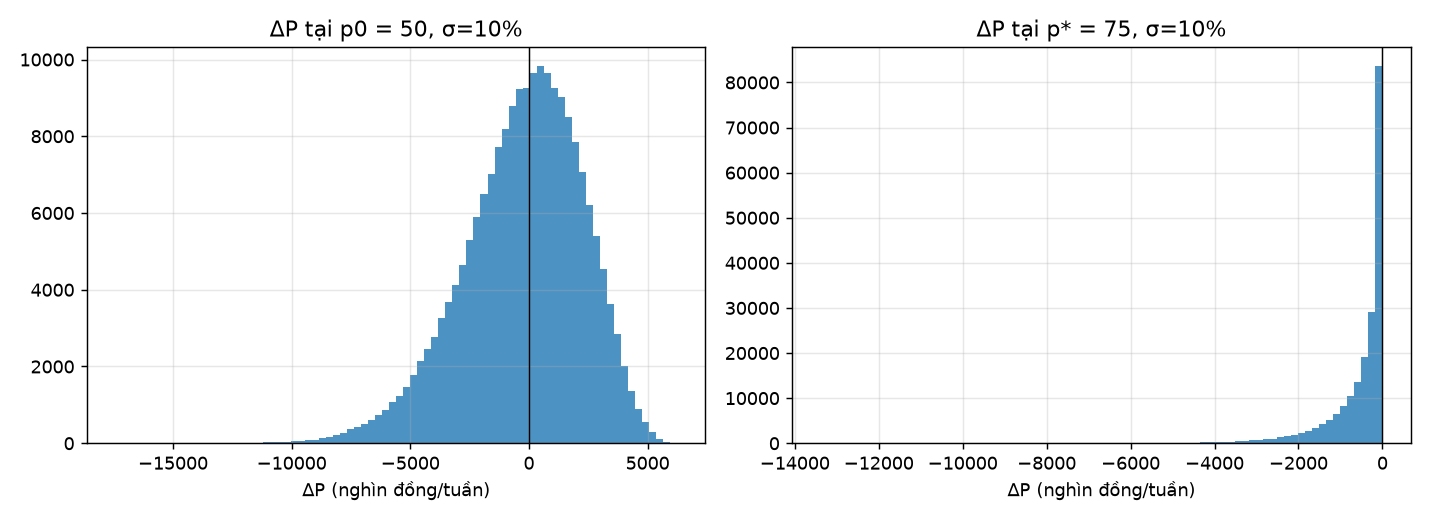
\includegraphics[width=\textwidth]{TN6_montecarlo_hist.png}
\caption{Phân bố của $\Delta P$ ở mô hình (L), $\sigma=10\%$: tại $p_0$ (trái) và tại $p^*$ (phải).}\label{fig:tn6}
\end{figure}

\subsection{TN7: Vùng tin cậy của vi phân}
Bảng~\ref{tab:tn7} cho mức lệch giá lớn nhất (tính theo $\%$ của $p_0$, dạng ``tăng\,/\,giảm'') để
$E_{\mathrm{rel}}\le\tau$; ``$\geq 50$'' nghĩa là không chạm ngưỡng trong khoảng khảo sát.

\begin{table}[ht]
\tbsty
\caption{Vùng tin cậy của vi phân (đơn vị: $\%$ của $p_0$).}\label{tab:tn7}
% Tự sinh bởi make_tables.py - không sửa tay.

\begin{tabular}{@{}llcccc@{}}
\toprule
Mô hình & Đại lượng & Điểm & $\tau=1\%$ & $\tau=5\%$ & $\tau=10\%$ \\
\midrule
Tuyến tính (L) & $q$ & $p_0$ & $\geq 50$ & $\geq 50$ & $\geq 50$ \\
 & $R$ & $p_0$ & ${+}0{,}35\,/\,{-}0{,}40$ & ${+}1{,}90\,/\,{-}2{,}10$ & ${+}3{,}60\,/\,{-}4{,}40$ \\
 & $P$ & $p_0$ & ${+}0{,}95\,/\,{-}1{,}00$ & ${+}4{,}75\,/\,{-}5{,}25$ & ${+}9{,}05\,/\,{-}11{,}10$ \\
 & $P$ & $p^*$ & ${+}0{,}00\,/\,{-}0{,}00$ & ${+}0{,}00\,/\,{-}0{,}00$ & ${+}0{,}00\,/\,{-}0{,}00$ \\
\midrule
Co giãn (E) & $q$ & $p_0$ & ${+}0{,}65\,/\,{-}0{,}65$ & ${+}3{,}30\,/\,{-}3{,}35$ & ${+}6{,}55\,/\,{-}6{,}70$ \\
 & $R$ & $p_0$ & ${+}0{,}95\,/\,{-}1{,}00$ & ${+}5{,}00\,/\,{-}5{,}00$ & ${+}9{,}95\,/\,{-}10{,}00$ \\
 & $P$ & $p_0$ & ${+}0{,}35\,/\,{-}0{,}40$ & ${+}1{,}95\,/\,{-}2{,}00$ & ${+}3{,}85\,/\,{-}4{,}15$ \\
 & $P$ & $p^*$ & ${+}0{,}00\,/\,{-}0{,}00$ & ${+}0{,}00\,/\,{-}0{,}00$ & ${+}0{,}00\,/\,{-}0{,}00$ \\
\bottomrule
\end{tabular}

\end{table}

Vùng tin cậy tăng xấp xỉ tỉ lệ với $\tau$ (ví dụ $P$ ở (L): $0{,}95$; $4{,}75$; $9{,}05$ cho $\tau=1;5;10\%$),
đúng như ước lượng~\eqref{eq:safe}. Với cùng $\tau=5\%$, ở (L) $R$ có vùng hẹp nhất ($+1{,}90/-2{,}10$)
còn $q$ chính xác tuyệt đối, trong khi ở (E) $P$ hẹp nhất ($+1{,}95/-2{,}00$). Tại $p^*$ vùng bằng $0$.

\begin{figure}[ht]
\centering
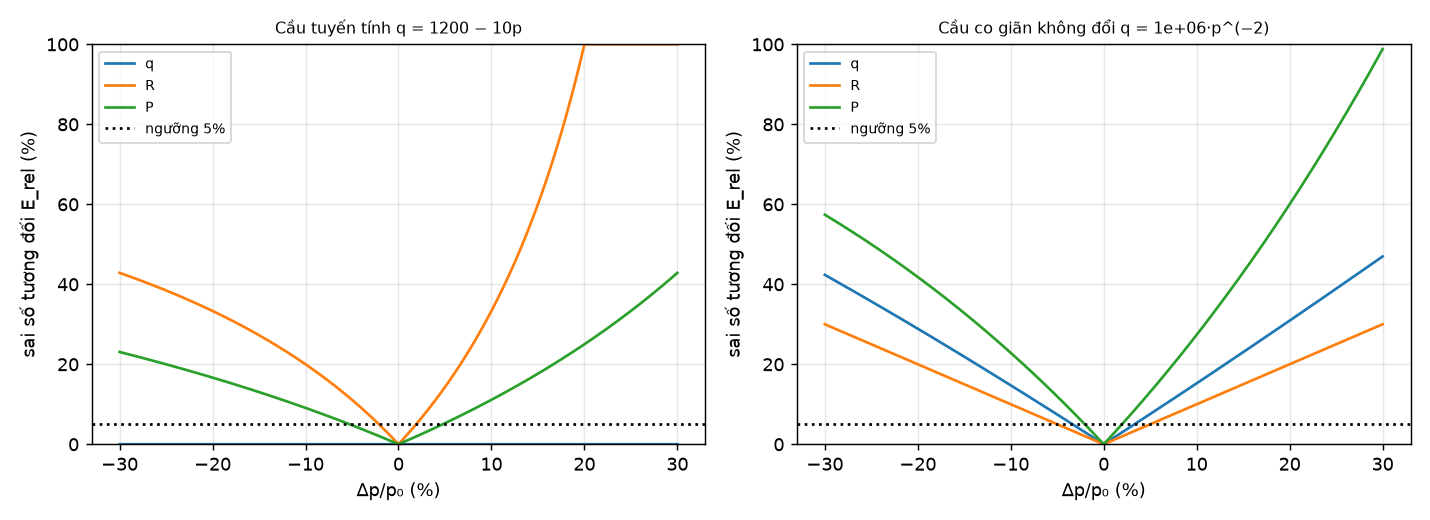
\includegraphics[width=\textwidth]{TN7_erel_vs_delta.png}
\caption{$E_{\mathrm{rel}}$ theo $\Delta p/p_0$ tại $p_0$ (đường chấm: ngưỡng $5\%$).}\label{fig:tn7}
\end{figure}

\subsection{TN8: Xấp xỉ bậc hai}
Bảng~\ref{tab:tn8} so sánh vi phân bậc một $dP$ và xấp xỉ bậc hai $dP_2$ cho $P$ ở mô hình (E).
Ở mô hình (L), $R$ và $P$ là đa thức bậc hai nên $dP_2$ trùng $\Delta P$ ở mọi dòng (sai số $0$).

\begin{table}[ht]
\tbsty
\caption{Mô hình (E): $P$ tại $p_0=40$ và $p^*=60$, xấp xỉ bậc một và bậc hai.}\label{tab:tn8}
{\setlength{\tabcolsep}{5pt}% Tự sinh bởi make_tables.py - không sửa tay.

\begin{tabular}{@{}clrrrrr@{}}
\toprule
Điểm & $\Delta p/p_0$ (\%) & $\Delta P$ thực & $dP$ (bậc 1) & $dP_2$ (bậc 2) & $E_{\mathrm{rel}}$ bậc 1 (\%) & $E_{\mathrm{rel}}$ bậc 2 (\%) \\
\midrule
$p_0$ & ${-}20$ & ${-}4\,296{,}9$ & ${-}2\,500{,}0$ & ${-}3\,750{,}0$ & $41{,}82$ & $12{,}73$ \\
 & ${-}10$ & ${-}1\,620{,}4$ & ${-}1\,250{,}0$ & ${-}1\,562{,}5$ & $22{,}86$ & $3{,}57$ \\
 & ${-}5$ & ${-}709{,}8$ & ${-}625{,}0$ & ${-}703{,}1$ & $11{,}95$ & $0{,}95$ \\
 & ${+}5$ & $552{,}7$ & $625{,}0$ & $546{,}9$ & $13{,}08$ & $1{,}06$ \\
 & ${+}10$ & $981{,}4$ & $1\,250{,}0$ & $937{,}5$ & $27{,}37$ & $4{,}47$ \\
 & ${+}20$ & $1\,562{,}5$ & $2\,500{,}0$ & $1\,250{,}0$ & $60{,}00$ & $20{,}00$ \\
\midrule
$p^*$ & ${-}20$ & ${-}520{,}8$ & $0{,}0$ & ${-}333{,}3$ & $100{,}00$ & $36{,}00$ \\
 & ${-}10$ & ${-}102{,}9$ & $0{,}0$ & ${-}83{,}3$ & $100{,}00$ & $19{,}00$ \\
 & ${-}5$ & ${-}23{,}1$ & $0{,}0$ & ${-}20{,}8$ & $100{,}00$ & $9{,}75$ \\
 & ${+}5$ & ${-}18{,}9$ & $0{,}0$ & ${-}20{,}8$ & $100{,}00$ & $10{,}25$ \\
 & ${+}10$ & ${-}68{,}9$ & $0{,}0$ & ${-}83{,}3$ & $100{,}00$ & $21{,}00$ \\
 & ${+}20$ & ${-}231{,}5$ & $0{,}0$ & ${-}333{,}3$ & $100{,}00$ & $44{,}00$ \\
\bottomrule
\end{tabular}
}
\end{table}

Tại $p_0$ với $\Delta p/p_0=+5\%$, $E_{\mathrm{rel}}$ giảm từ $13{,}08\%$ xuống $1{,}06\%$; với $+10\%$ từ
$27{,}37\%$ xuống $4{,}47\%$; với $+20\%$ từ $60{,}00\%$ xuống $20{,}00\%$. Tại $p^*$, vi phân bậc một cho
$dP=0$ ($E_{\mathrm{rel}}=100\%$) còn $dP_2$ bắt được thay đổi thực với sai số $10{,}25\%$ ($+5\%$) và
$9{,}75\%$ ($-5\%$). Hệ số góc log-log (Bảng~\ref{tab:tn8o}, Hình~\ref{fig:tn8}) xấp xỉ $2$ cho bậc một và
xấp xỉ $3$ cho bậc hai ($2{,}95$ đến $2{,}96$ ở mô hình E), khớp với lý thuyết ở Mục~\ref{sec:phuongphap}.

\begin{table}[ht]
\tbsty
\caption{Hệ số góc log-log của sai số xấp xỉ bậc một và bậc hai. Dấu ``---'': sai số bằng $0$.}\label{tab:tn8o}
% Tự sinh bởi make_tables.py - không sửa tay.

\begin{tabular}{@{}llcrr@{}}
\toprule
Mô hình & Đại lượng & Điểm & Bậc 1 & Bậc 2 \\
\midrule
Tuyến tính (L) & $R$ & $p_0$ & $2{,}000$ & --- \\
 & $P$ & $p_0$ & $2{,}000$ & --- \\
 & $P$ & $p^*$ & $2{,}000$ & --- \\
\midrule
Co giãn (E) & $R$ & $p_0$ & $1{,}980$ & $2{,}964$ \\
 & $P$ & $p_0$ & $1{,}968$ & $2{,}960$ \\
 & $P$ & $p^*$ & $1{,}959$ & $2{,}950$ \\
\bottomrule
\end{tabular}

\end{table}

\begin{figure}[ht]
\centering
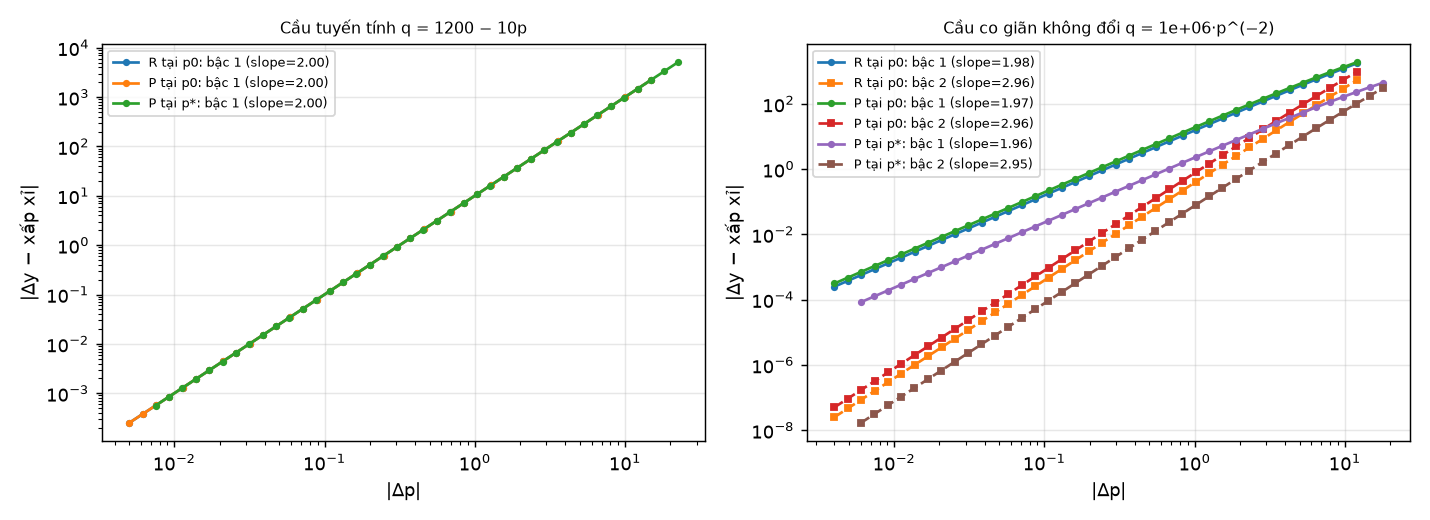
\includegraphics[width=\textwidth]{TN8_second_order_loglog.png}
\caption{Sai số của xấp xỉ bậc một và bậc hai theo $|\Delta p|$ (log-log).}\label{fig:tn8}
\end{figure}
.
% Cần: amsmath, booktabs, graphicx. Bảng nằm trong generated/ (tự sinh bởi
% make_tables.py từ output/tables), hình nằm trong ../output/figures.
% Chỉ nêu SỐ LIỆU quan sát được; phần diễn giải ý nghĩa thuộc Mục kết quả và phân tích.
% ============================================================
\section{Tính toán, mô phỏng và thực nghiệm}\label{sec:thucnghiem}

\subsection{Cài đặt và kiểm chứng}
Chương trình được viết bằng Python (NumPy, pandas, Matplotlib) và chia thành các tệp
riêng: \texttt{src/model.py} (hai mô hình cầu và các đạo hàm tính tay),
\texttt{src/sensitivity.py} (thay đổi thực, vi phân, sai số, độ nhạy, bậc hội tụ, xấp xỉ
bậc hai, vùng tin cậy), \texttt{src/montecarlo.py} (mô phỏng nhiễu giá),
\texttt{experiments.py} (chạy các thí nghiệm, xuất bảng CSV và hình PNG) và
\texttt{app.py} (ứng dụng tương tác dùng chung mã với báo cáo). Phần mềm chỉ dùng để
tính toán, vẽ đồ thị và kiểm chứng: mọi đạo hàm và công thức sai số được cài đặt từ
các biểu thức ở Mục~\ref{sec:phuongphap}, không gọi hàm có sẵn để tạo kết quả chính.

Việc kiểm chứng do \texttt{verify.py} thực hiện: với $40$ điểm trong miền xác định, các hàm
$q,R,P$ và đạo hàm cấp một, cấp hai cài đặt trong chương trình khớp SymPy với sai lệch
tương đối nhỏ hơn $10^{-9}$, và đạo hàm cấp một khớp sai phân trung tâm với sai lệch
tương đối nhỏ hơn $10^{-5}$; ngoài ra $P'(p^*)=0$ với sai số dưới $10^{-8}$.
Mọi số liệu dưới đây được sinh lại bằng một lệnh (\texttt{uv run experiments.py}) với hạt
giống mô phỏng cố định, nên chạy lại cho kết quả giống hệt.

Tám thí nghiệm (TN) được thực hiện trên hai mô hình ở Bảng~\ref{tab:par}:

\begin{table}[ht]
\tbsty
\caption{Các thí nghiệm và công cụ Giải tích tương ứng.}\label{tab:tn}
\begin{tabular}{@{}l p{6.2cm} p{6.2cm}@{}}
\toprule
TN & Câu hỏi & Công cụ \\
\midrule
1 & Vi phân dự báo thay đổi thực tốt đến đâu? & vi phân, sai số tuyệt đối/tương đối \\
2 & Xấp xỉ tuyến tính trông thế nào? & tiếp tuyến \\
3 & Sai số giảm theo $\Delta p$ với bậc bao nhiêu? & khai triển Taylor, hồi quy log-log \\
4 & Đại lượng nào nhạy nhất với giá? & độ nhạy tương đối $S$ \\
5 & Kết quả có đổi khi đổi tham số mô hình không? & quét $b$ (L) và $k$ (E) \\
6 & Giá nhiễu ngẫu nhiên thì $\Delta P$ phân bố ra sao? & Monte Carlo, Taylor \\
7 & Vi phân dùng được đến mức lệch giá nào? & vùng tin cậy theo ngưỡng $\tau$ \\
8 & Thêm số hạng bậc hai cải thiện bao nhiêu? & xấp xỉ Taylor bậc hai \\
\bottomrule
\end{tabular}
\end{table}

\subsection{TN1: So sánh thay đổi thực và vi phân}
Với mỗi mức lệch $\Delta p/p_0\in\{\pm1,\pm2,\pm5,\pm10,\pm20\}\%$ ta tính $\Delta P$ thực,
$dP=P'(p_0)\Delta p$ và sai số (Bảng~\ref{tab:tn1l} và~\ref{tab:tn1e}; đơn vị của $\Delta P$,
$dP$ là nghìn đồng/tuần).

\begin{table}[ht]
\tbsty
\caption{Lợi nhuận $P$ tại $p_0=50$, mô hình (L).}\label{tab:tn1l}
% Tự sinh bởi make_tables.py - không sửa tay.

\begin{tabular}{@{}rrrrr@{}}
\toprule
$\Delta p/p_0$ (\%) & $\Delta P$ thực & $dP$ & $|\Delta P-dP|$ & $E_{\mathrm{rel}}$ (\%) \\
\midrule
${-}20$ & ${-}6\,000{,}0$ & ${-}5\,000{,}0$ & $1\,000{,}0$ & $16{,}67$ \\
${-}10$ & ${-}2\,750{,}0$ & ${-}2\,500{,}0$ & $250{,}0$ & $9{,}09$ \\
${-}5$ & ${-}1\,312{,}5$ & ${-}1\,250{,}0$ & $62{,}5$ & $4{,}76$ \\
${-}2$ & ${-}510{,}0$ & ${-}500{,}0$ & $10{,}0$ & $1{,}96$ \\
${-}1$ & ${-}252{,}5$ & ${-}250{,}0$ & $2{,}5$ & $0{,}99$ \\
${+}1$ & $247{,}5$ & $250{,}0$ & $2{,}5$ & $1{,}01$ \\
${+}2$ & $490{,}0$ & $500{,}0$ & $10{,}0$ & $2{,}04$ \\
${+}5$ & $1\,187{,}5$ & $1\,250{,}0$ & $62{,}5$ & $5{,}26$ \\
${+}10$ & $2\,250{,}0$ & $2\,500{,}0$ & $250{,}0$ & $11{,}11$ \\
${+}20$ & $4\,000{,}0$ & $5\,000{,}0$ & $1\,000{,}0$ & $25{,}00$ \\
\bottomrule
\end{tabular}

\end{table}

\begin{table}[ht]
\tbsty
\caption{Lợi nhuận $P$ tại $p_0=40$, mô hình (E).}\label{tab:tn1e}
% Tự sinh bởi make_tables.py - không sửa tay.

\begin{tabular}{@{}rrrrr@{}}
\toprule
$\Delta p/p_0$ (\%) & $\Delta P$ thực & $dP$ & $|\Delta P-dP|$ & $E_{\mathrm{rel}}$ (\%) \\
\midrule
${-}20$ & ${-}4\,296{,}9$ & ${-}2\,500{,}0$ & $1\,796{,}9$ & $41{,}82$ \\
${-}10$ & ${-}1\,620{,}4$ & ${-}1\,250{,}0$ & $370{,}4$ & $22{,}86$ \\
${-}5$ & ${-}709{,}8$ & ${-}625{,}0$ & $84{,}8$ & $11{,}95$ \\
${-}2$ & ${-}262{,}9$ & ${-}250{,}0$ & $12{,}9$ & $4{,}91$ \\
${-}1$ & ${-}128{,}2$ & ${-}125{,}0$ & $3{,}2$ & $2{,}48$ \\
${+}1$ & $121{,}9$ & $125{,}0$ & $3{,}1$ & $2{,}52$ \\
${+}2$ & $237{,}9$ & $250{,}0$ & $12{,}1$ & $5{,}09$ \\
${+}5$ & $552{,}7$ & $625{,}0$ & $72{,}3$ & $13{,}08$ \\
${+}10$ & $981{,}4$ & $1\,250{,}0$ & $268{,}6$ & $27{,}37$ \\
${+}20$ & $1\,562{,}5$ & $2\,500{,}0$ & $937{,}5$ & $60{,}00$ \\
\bottomrule
\end{tabular}

\end{table}

Ở mô hình (L), $E_{\mathrm{rel}}$ tăng từ $1{,}0\%$ ($\Delta p/p_0=\pm1\%$) lên $5{,}3\%$
($+5\%$) và $25{,}0\%$ ($+20\%$); ở mô hình (E) từ $2{,}5\%$ lên $13{,}1\%$ và $60{,}0\%$. Với
(L), $P$ là hàm bậc hai nên $|\Delta P-dP|=\tfrac12|P''|\Delta p^2$ đối xứng giữa hai phía
(ví dụ $62{,}5$ cho cả $\pm5\%$), còn $E_{\mathrm{rel}}$ không đối xứng ($4{,}76\%$ và $5{,}26\%$)
vì $\Delta P$ ở hai phía khác nhau.

Tại giá tối ưu $p^*$ (với $P'(p^*)=0$) thì $dP=0$; thay đổi thực khi giá tăng $5\%$ là
$-140{,}6$ (mô hình L, $p^*=75$) và $-18{,}9$ (mô hình E, $p^*=60$), nên $E_{\mathrm{rel}}=100\%$.
Với $q$ và $R$, kết quả tương tự được lưu trong \texttt{output/tables/}.

\subsection{TN2: Tiếp tuyến và đường cong}
Hình~\ref{fig:tn2l} và~\ref{fig:tn2e} vẽ $q,R,P$ cùng tiếp tuyến tại $p_0$; dải tô màu là
$p_0\pm20\%$. Khoảng cách giữa đường cong và tiếp tuyến chính là sai số của xấp xỉ vi phân,
nhỏ gần $p_0$ và tăng nhanh khi ra xa.

\begin{figure}[ht]
\centering
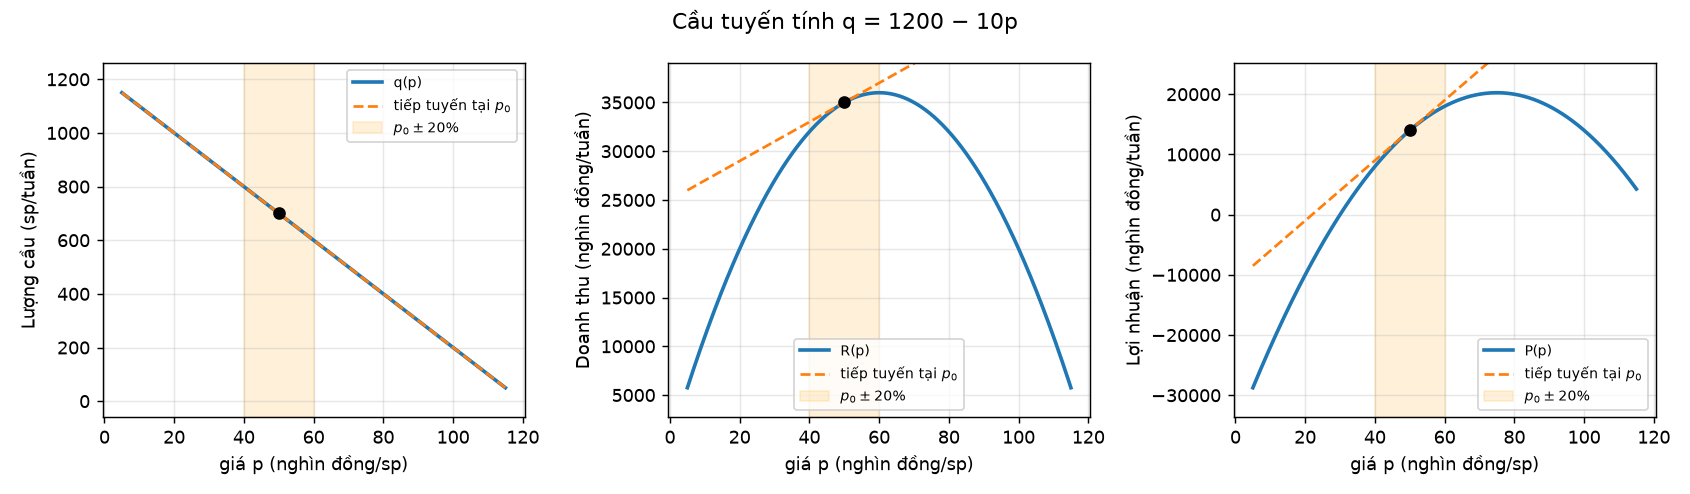
\includegraphics[width=\textwidth]{TN2_tangent_linear.png}
\caption{Mô hình (L): $q$, $R$, $P$ và tiếp tuyến tại $p_0=50$.}\label{fig:tn2l}
\end{figure}
\begin{figure}[ht]
\centering
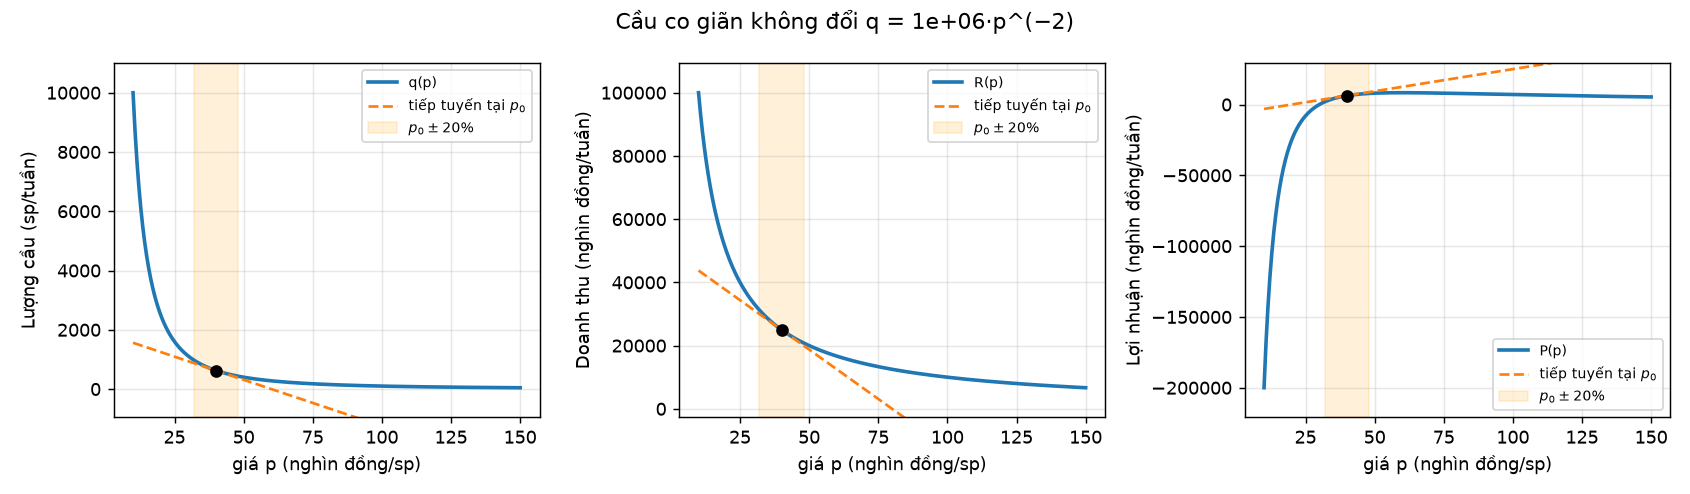
\includegraphics[width=\textwidth]{TN2_tangent_elastic.png}
\caption{Mô hình (E): $q$, $R$, $P$ và tiếp tuyến tại $p_0=40$.}\label{fig:tn2e}
\end{figure}

\subsection{TN3: Bậc của sai số}
Hệ số góc log-log của $E_{\mathrm{abs}}$ theo $|\Delta p|$ (cách đo ở Mục~\ref{sec:phuongphap}) cho trong
Bảng~\ref{tab:tn3}; kỳ vọng là $2$.

\begin{table}[ht]
\tbsty
\caption{Hệ số góc log-log của sai số vi phân. Dấu ``---'': sai số bằng $0$.}\label{tab:tn3}
% Tự sinh bởi make_tables.py - không sửa tay.

\begin{tabular}{@{}llcr@{}}
\toprule
Mô hình & Đại lượng & Điểm & Hệ số góc log-log \\
\midrule
Tuyến tính (L) & $q$ & $p_0$ & --- \\
 & $R$ & $p_0$ & $2{,}000$ \\
 & $P$ & $p_0$ & $2{,}000$ \\
 & $P$ & $p^*$ & $2{,}000$ \\
\midrule
Co giãn (E) & $q$ & $p_0$ & $1{,}973$ \\
 & $R$ & $p_0$ & $1{,}980$ \\
 & $P$ & $p_0$ & $1{,}968$ \\
 & $P$ & $p^*$ & $1{,}959$ \\
\bottomrule
\end{tabular}

\end{table}

Ở (L), $R$ và $P$ cho đúng $2{,}000$, còn $q$ là hàm tuyến tính nên sai số bằng $0$. Ở (E), các
hệ số góc nằm trong khoảng $1{,}96$ đến $1{,}98$, gần $2$ nhưng hơi lệch vì lưới $\Delta p$ trải đến
$30\%$ nên các số hạng bậc cao bắt đầu có ảnh hưởng (Hình~\ref{fig:tn3}).

\begin{figure}[ht]
\centering
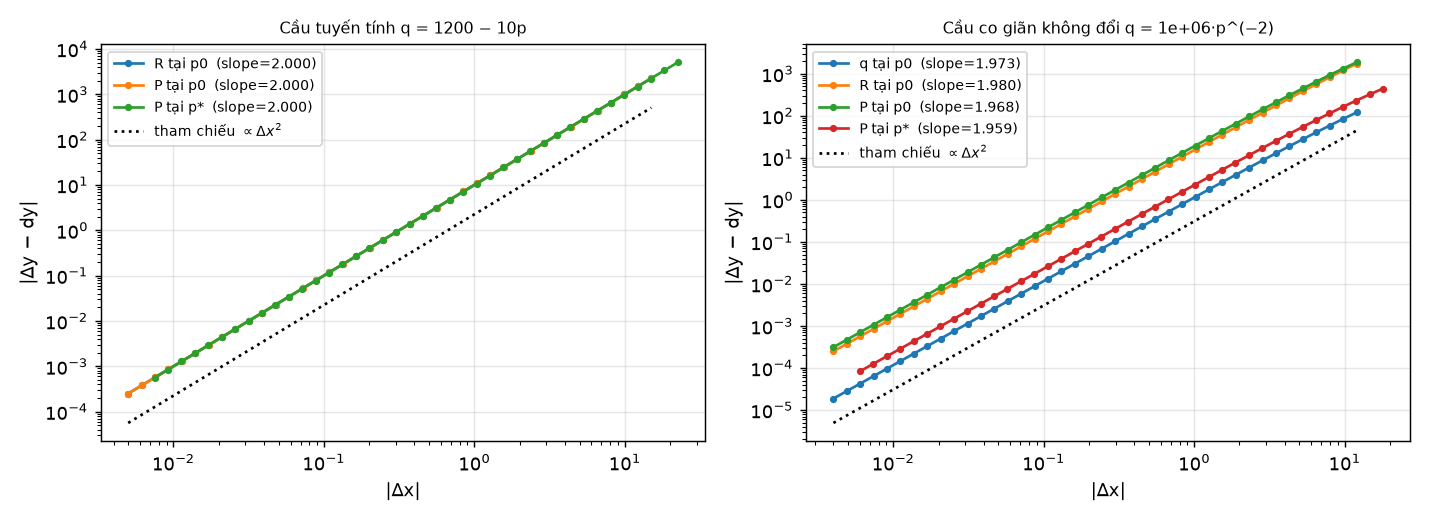
\includegraphics[width=\textwidth]{TN3_error_loglog.png}
\caption{Sai số $|\Delta y-dy|$ theo $|\Delta p|$ (thang log-log) và đường tham chiếu $\propto\Delta p^2$.}\label{fig:tn3}
\end{figure}

\subsection{TN4: Độ nhạy tương đối}
Bảng~\ref{tab:tn4} cho $S=f'p/f$ tại $p_0$ và $p^*$; Hình~\ref{fig:tn4} vẽ $S(p)$ (cắt ở $|S|>12$).

\begin{table}[ht]
\tbsty
\caption{Độ nhạy tương đối của $q$, $R$, $P$ theo giá.}\label{tab:tn4}
% Tự sinh bởi make_tables.py - không sửa tay.

\begin{tabular}{@{}llrr@{}}
\toprule
Mô hình & Độ nhạy & tại $p_0$ & tại $p^*$ \\
\midrule
Tuyến tính (L) & $S_q$ & ${-}0{,}714$ & ${-}1{,}667$ \\
 & $S_R$ & $0{,}286$ & ${-}0{,}667$ \\
 & $S_P$ & $1{,}786$ & $0{,}000$ \\
\midrule
Co giãn (E) & $S_q$ & ${-}2{,}000$ & ${-}2{,}000$ \\
 & $S_R$ & ${-}1{,}000$ & ${-}1{,}000$ \\
 & $S_P$ & $2{,}000$ & $0{,}000$ \\
\bottomrule
\end{tabular}

\end{table}

Tại $p_0$, ở (L) $|S_P|=1{,}786$ lớn nhất, sau đó là $|S_q|=0{,}714$ và $|S_R|=0{,}286$; ở (E)
$S_q=-2$, $S_R=-1$, $S_P=2$, trong đó $|S_P|$ và $|S_q|$ bằng nhau. Các giá trị khớp với hệ
thức~\eqref{eq:S}: ví dụ ở (L), $S_P=50/20-0{,}714=1{,}786$; ở (E), $S_P=40/10-2=2$. Tại $p^*$,
$S_P=0$ ở cả hai mô hình.

\begin{figure}[ht]
\centering
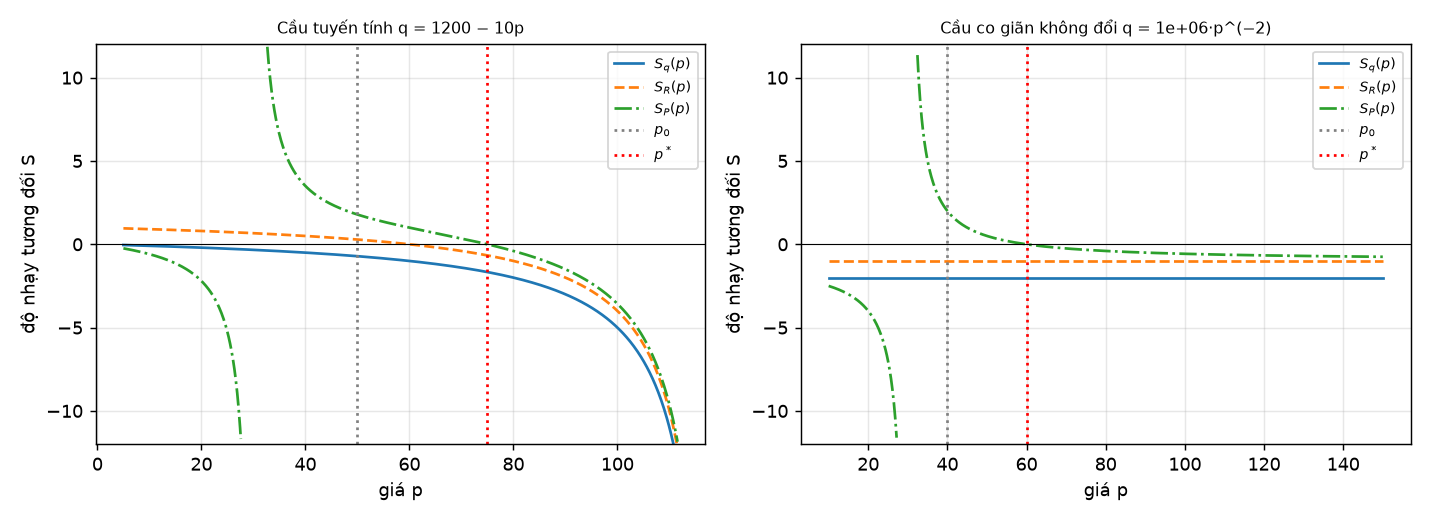
\includegraphics[width=\textwidth]{TN4_elasticity.png}
\caption{Độ nhạy $S_q$, $S_R$, $S_P$ theo giá $p$ (đường chấm: $p_0$ và $p^*$).}\label{fig:tn4}
\end{figure}

\subsection{TN5: Ảnh hưởng của tham số mô hình}
Cố định $\Delta p=+10\%$ và thay đổi độ dốc cầu $b$ (mô hình L) hoặc độ co giãn $k$ (mô hình E); các
bảng cho $E_{\mathrm{rel}}$ của $q$, $R$, $P$.

\begin{center}
\linespread{1}\small\selectfont
\begin{minipage}[t]{0.48\textwidth}\centering
\captionof{table}{Mô hình (L): $E_{\mathrm{rel}}$ (\%) khi thay đổi $b$.}\label{tab:tn5l}
% Tự sinh bởi make_tables.py - không sửa tay.

\begin{tabular}{@{}rrrr@{}}
\toprule
$b$ & $q$ & $R$ & $P$ \\
\midrule
$5{,}0$ & $0{,}0$ & $3{,}7$ & $3{,}0$ \\
$7{,}5$ & $0{,}0$ & $9{,}1$ & $5{,}9$ \\
$10{,}0$ & $0{,}0$ & $33{,}3$ & $11{,}1$ \\
$12{,}5$ & $0{,}0$ & $55{,}6$ & $23{,}8$ \\
$15{,}0$ & $0{,}0$ & $20{,}0$ & $100{,}0$ \\
$17{,}5$ & $0{,}0$ & $13{,}7$ & $77{,}8$ \\
$20{,}0$ & $0{,}0$ & $11{,}1$ & $33{,}3$ \\
\bottomrule
\end{tabular}

\end{minipage}\hfill
\begin{minipage}[t]{0.48\textwidth}\centering
\captionof{table}{Mô hình (E): $E_{\mathrm{rel}}$ (\%) khi thay đổi $k$.}\label{tab:tn5e}
% Tự sinh bởi make_tables.py - không sửa tay.

\begin{tabular}{@{}rrrr@{}}
\toprule
$k$ & $q$ & $R$ & $P$ \\
\midrule
$1{,}2$ & $11{,}0$ & $5{,}9$ & $12{,}6$ \\
$1{,}5$ & $12{,}6$ & $7{,}4$ & $17{,}1$ \\
$2{,}0$ & $15{,}2$ & $10{,}0$ & $27{,}4$ \\
$2{,}5$ & $17{,}9$ & $12{,}6$ & $45{,}4$ \\
$3{,}0$ & $20{,}6$ & $15{,}2$ & $92{,}9$ \\
$4{,}0$ & $26{,}2$ & $20{,}6$ & $100{,}0$ \\
\bottomrule
\end{tabular}

\end{minipage}
\end{center}

\begin{figure}[ht]
\centering
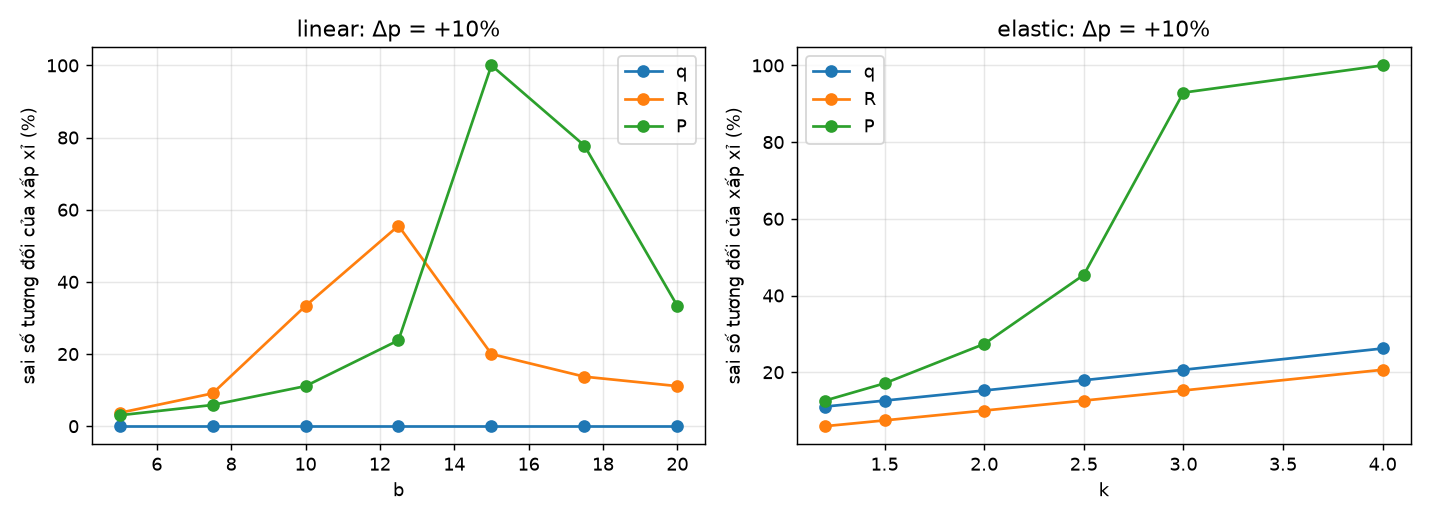
\includegraphics[width=\textwidth]{TN5_param_study.png}
\caption{Sai số tương đối của xấp xỉ vi phân khi $\Delta p=+10\%$ theo tham số mô hình.}\label{fig:tn5}
\end{figure}

Ở (L), $q$ luôn có sai số $0$. Sai số của $P$ không đơn điệu theo $b$: nó đạt $100\%$ tại $b=15$, vì khi
đó $p^*=(a+bc)/(2b)=55$ đúng bằng giá mới $p_0+10\%$, nên $\Delta P=dP/2$. Sai số của $R$ lớn nhất ở
$b=12{,}5$, gần $b=12$ là lúc $R'(p_0)=a-2bp_0=0$. Ở (E), sai số của cả ba đại lượng tăng theo $k$;
$P$ đạt $100\%$ tại $k=4$ vì khi đó $p^*=ck/(k-1)=40=p_0$, tức $P'(p_0)=0$ và $dP=0$.

\subsection{TN6: Mô phỏng Monte Carlo}
Giá thực tế $p=p_0(1+\varepsilon)$, $\varepsilon\sim N(0,\sigma^2)$, $N=200\,000$ mẫu, hạt giống
$20260503$. Bảng~\ref{tab:tn6} so sánh trung bình và độ lệch chuẩn của $\Delta P$ với
dự đoán~\eqref{eq:mc} (đơn vị nghìn đồng/tuần); Hình~\ref{fig:tn6} là phân bố của $\Delta P$ ở mô hình (L)
với $\sigma=10\%$.

\begin{table}[ht]
\tbsty
\caption{Monte Carlo: $\Delta P$ thực và dự đoán từ khai triển Taylor.}\label{tab:tn6}
{\setlength{\tabcolsep}{5pt}% Tự sinh bởi make_tables.py - không sửa tay.

\begin{tabular}{@{}llcrrrr@{}}
\toprule
Mô hình & Điểm & $\sigma$ (\%) & std thực & std dự đoán & mean thực & mean dự đoán \\
\midrule
Tuyến tính (L) & $p_0$ & $1$ & $248{,}50$ & $250{,}00$ & ${-}3{,}36$ & ${-}2{,}50$ \\
 & $p_0$ & $5$ & $1\,245{,}70$ & $1\,250{,}00$ & ${-}66{,}17$ & ${-}62{,}50$ \\
 & $p_0$ & $10$ & $2\,510{,}27$ & $2\,500{,}00$ & ${-}255{,}82$ & ${-}250{,}00$ \\
 & $p^*$ & $1$ & $7{,}85$ & $0{,}00$ & ${-}5{,}56$ & ${-}5{,}62$ \\
 & $p^*$ & $5$ & $196{,}22$ & $0{,}00$ & ${-}138{,}91$ & ${-}140{,}62$ \\
 & $p^*$ & $10$ & $784{,}86$ & $0{,}00$ & ${-}555{,}63$ & ${-}562{,}50$ \\
\midrule
Co giãn (E) & $p_0$ & $1$ & $124{,}47$ & $125{,}00$ & ${-}3{,}53$ & ${-}3{,}12$ \\
 & $p_0$ & $5$ & $650{,}40$ & $625{,}00$ & ${-}80{,}72$ & ${-}78{,}12$ \\
 & $p_0$ & $10$ & $1\,499{,}47$ & $1\,250{,}00$ & ${-}335{,}37$ & ${-}312{,}50$ \\
 & $p^*$ & $1$ & $1{,}17$ & $0{,}00$ & ${-}0{,}82$ & ${-}0{,}83$ \\
 & $p^*$ & $5$ & $31{,}55$ & $0{,}00$ & ${-}21{,}06$ & ${-}20{,}83$ \\
 & $p^*$ & $10$ & $159{,}18$ & $0{,}00$ & ${-}90{,}44$ & ${-}83{,}33$ \\
\bottomrule
\end{tabular}
}
\end{table}

Tại $p_0$, độ lệch chuẩn mô phỏng sát dự đoán $|P'|p_0\sigma$ (ví dụ $248{,}5$ so với $250{,}0$ ở (L),
$\sigma=1\%$), và trung bình âm sát $\tfrac12P''(p_0\sigma)^2$; độ lệch tăng khi $\sigma$ lớn ở mô
hình (E) ($1\,499$ so với $1\,250$ khi $\sigma=10\%$). Tại $p^*$ dự đoán bậc nhất của độ lệch chuẩn
bằng $0$ nhưng mô phỏng cho giá trị dương và trung bình âm, phù hợp với $\Delta P\approx\tfrac12P''(p^*\varepsilon)^2\le0$:
với $\sigma=5\%$, công thức $|P''|(p^*\sigma)^2/\sqrt2$ cho $198{,}9$ (L) và $29{,}5$ (E), so với $196{,}2$ và
$31{,}5$ mô phỏng.

\begin{figure}[ht]
\centering
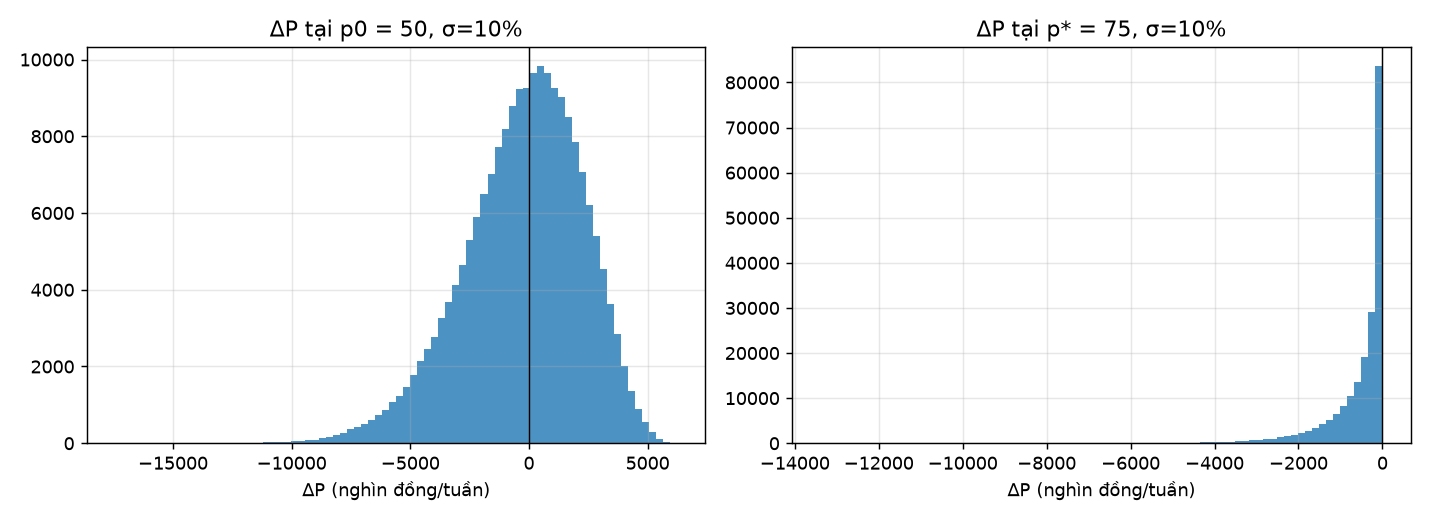
\includegraphics[width=\textwidth]{TN6_montecarlo_hist.png}
\caption{Phân bố của $\Delta P$ ở mô hình (L), $\sigma=10\%$: tại $p_0$ (trái) và tại $p^*$ (phải).}\label{fig:tn6}
\end{figure}

\subsection{TN7: Vùng tin cậy của vi phân}
Bảng~\ref{tab:tn7} cho mức lệch giá lớn nhất (tính theo $\%$ của $p_0$, dạng ``tăng\,/\,giảm'') để
$E_{\mathrm{rel}}\le\tau$; ``$\geq 50$'' nghĩa là không chạm ngưỡng trong khoảng khảo sát.

\begin{table}[ht]
\tbsty
\caption{Vùng tin cậy của vi phân (đơn vị: $\%$ của $p_0$).}\label{tab:tn7}
% Tự sinh bởi make_tables.py - không sửa tay.

\begin{tabular}{@{}llcccc@{}}
\toprule
Mô hình & Đại lượng & Điểm & $\tau=1\%$ & $\tau=5\%$ & $\tau=10\%$ \\
\midrule
Tuyến tính (L) & $q$ & $p_0$ & $\geq 50$ & $\geq 50$ & $\geq 50$ \\
 & $R$ & $p_0$ & ${+}0{,}35\,/\,{-}0{,}40$ & ${+}1{,}90\,/\,{-}2{,}10$ & ${+}3{,}60\,/\,{-}4{,}40$ \\
 & $P$ & $p_0$ & ${+}0{,}95\,/\,{-}1{,}00$ & ${+}4{,}75\,/\,{-}5{,}25$ & ${+}9{,}05\,/\,{-}11{,}10$ \\
 & $P$ & $p^*$ & ${+}0{,}00\,/\,{-}0{,}00$ & ${+}0{,}00\,/\,{-}0{,}00$ & ${+}0{,}00\,/\,{-}0{,}00$ \\
\midrule
Co giãn (E) & $q$ & $p_0$ & ${+}0{,}65\,/\,{-}0{,}65$ & ${+}3{,}30\,/\,{-}3{,}35$ & ${+}6{,}55\,/\,{-}6{,}70$ \\
 & $R$ & $p_0$ & ${+}0{,}95\,/\,{-}1{,}00$ & ${+}5{,}00\,/\,{-}5{,}00$ & ${+}9{,}95\,/\,{-}10{,}00$ \\
 & $P$ & $p_0$ & ${+}0{,}35\,/\,{-}0{,}40$ & ${+}1{,}95\,/\,{-}2{,}00$ & ${+}3{,}85\,/\,{-}4{,}15$ \\
 & $P$ & $p^*$ & ${+}0{,}00\,/\,{-}0{,}00$ & ${+}0{,}00\,/\,{-}0{,}00$ & ${+}0{,}00\,/\,{-}0{,}00$ \\
\bottomrule
\end{tabular}

\end{table}

Vùng tin cậy tăng xấp xỉ tỉ lệ với $\tau$ (ví dụ $P$ ở (L): $0{,}95$; $4{,}75$; $9{,}05$ cho $\tau=1;5;10\%$),
đúng như ước lượng~\eqref{eq:safe}. Với cùng $\tau=5\%$, ở (L) $R$ có vùng hẹp nhất ($+1{,}90/-2{,}10$)
còn $q$ chính xác tuyệt đối, trong khi ở (E) $P$ hẹp nhất ($+1{,}95/-2{,}00$). Tại $p^*$ vùng bằng $0$.

\begin{figure}[ht]
\centering
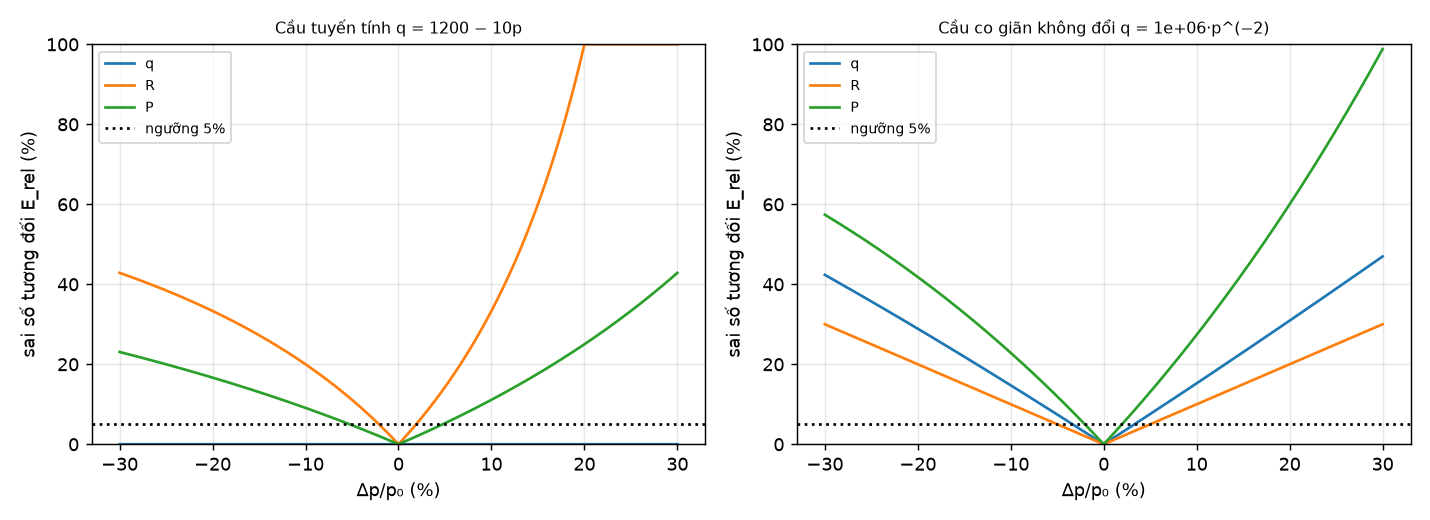
\includegraphics[width=\textwidth]{TN7_erel_vs_delta.png}
\caption{$E_{\mathrm{rel}}$ theo $\Delta p/p_0$ tại $p_0$ (đường chấm: ngưỡng $5\%$).}\label{fig:tn7}
\end{figure}

\subsection{TN8: Xấp xỉ bậc hai}
Bảng~\ref{tab:tn8} so sánh vi phân bậc một $dP$ và xấp xỉ bậc hai $dP_2$ cho $P$ ở mô hình (E).
Ở mô hình (L), $R$ và $P$ là đa thức bậc hai nên $dP_2$ trùng $\Delta P$ ở mọi dòng (sai số $0$).

\begin{table}[ht]
\tbsty
\caption{Mô hình (E): $P$ tại $p_0=40$ và $p^*=60$, xấp xỉ bậc một và bậc hai.}\label{tab:tn8}
{\setlength{\tabcolsep}{5pt}% Tự sinh bởi make_tables.py - không sửa tay.

\begin{tabular}{@{}clrrrrr@{}}
\toprule
Điểm & $\Delta p/p_0$ (\%) & $\Delta P$ thực & $dP$ (bậc 1) & $dP_2$ (bậc 2) & $E_{\mathrm{rel}}$ bậc 1 (\%) & $E_{\mathrm{rel}}$ bậc 2 (\%) \\
\midrule
$p_0$ & ${-}20$ & ${-}4\,296{,}9$ & ${-}2\,500{,}0$ & ${-}3\,750{,}0$ & $41{,}82$ & $12{,}73$ \\
 & ${-}10$ & ${-}1\,620{,}4$ & ${-}1\,250{,}0$ & ${-}1\,562{,}5$ & $22{,}86$ & $3{,}57$ \\
 & ${-}5$ & ${-}709{,}8$ & ${-}625{,}0$ & ${-}703{,}1$ & $11{,}95$ & $0{,}95$ \\
 & ${+}5$ & $552{,}7$ & $625{,}0$ & $546{,}9$ & $13{,}08$ & $1{,}06$ \\
 & ${+}10$ & $981{,}4$ & $1\,250{,}0$ & $937{,}5$ & $27{,}37$ & $4{,}47$ \\
 & ${+}20$ & $1\,562{,}5$ & $2\,500{,}0$ & $1\,250{,}0$ & $60{,}00$ & $20{,}00$ \\
\midrule
$p^*$ & ${-}20$ & ${-}520{,}8$ & $0{,}0$ & ${-}333{,}3$ & $100{,}00$ & $36{,}00$ \\
 & ${-}10$ & ${-}102{,}9$ & $0{,}0$ & ${-}83{,}3$ & $100{,}00$ & $19{,}00$ \\
 & ${-}5$ & ${-}23{,}1$ & $0{,}0$ & ${-}20{,}8$ & $100{,}00$ & $9{,}75$ \\
 & ${+}5$ & ${-}18{,}9$ & $0{,}0$ & ${-}20{,}8$ & $100{,}00$ & $10{,}25$ \\
 & ${+}10$ & ${-}68{,}9$ & $0{,}0$ & ${-}83{,}3$ & $100{,}00$ & $21{,}00$ \\
 & ${+}20$ & ${-}231{,}5$ & $0{,}0$ & ${-}333{,}3$ & $100{,}00$ & $44{,}00$ \\
\bottomrule
\end{tabular}
}
\end{table}

Tại $p_0$ với $\Delta p/p_0=+5\%$, $E_{\mathrm{rel}}$ giảm từ $13{,}08\%$ xuống $1{,}06\%$; với $+10\%$ từ
$27{,}37\%$ xuống $4{,}47\%$; với $+20\%$ từ $60{,}00\%$ xuống $20{,}00\%$. Tại $p^*$, vi phân bậc một cho
$dP=0$ ($E_{\mathrm{rel}}=100\%$) còn $dP_2$ bắt được thay đổi thực với sai số $10{,}25\%$ ($+5\%$) và
$9{,}75\%$ ($-5\%$). Hệ số góc log-log (Bảng~\ref{tab:tn8o}, Hình~\ref{fig:tn8}) xấp xỉ $2$ cho bậc một và
xấp xỉ $3$ cho bậc hai ($2{,}95$ đến $2{,}96$ ở mô hình E), khớp với lý thuyết ở Mục~\ref{sec:phuongphap}.

\begin{table}[ht]
\tbsty
\caption{Hệ số góc log-log của sai số xấp xỉ bậc một và bậc hai. Dấu ``---'': sai số bằng $0$.}\label{tab:tn8o}
% Tự sinh bởi make_tables.py - không sửa tay.

\begin{tabular}{@{}llcrr@{}}
\toprule
Mô hình & Đại lượng & Điểm & Bậc 1 & Bậc 2 \\
\midrule
Tuyến tính (L) & $R$ & $p_0$ & $2{,}000$ & --- \\
 & $P$ & $p_0$ & $2{,}000$ & --- \\
 & $P$ & $p^*$ & $2{,}000$ & --- \\
\midrule
Co giãn (E) & $R$ & $p_0$ & $1{,}980$ & $2{,}964$ \\
 & $P$ & $p_0$ & $1{,}968$ & $2{,}960$ \\
 & $P$ & $p^*$ & $1{,}959$ & $2{,}950$ \\
\bottomrule
\end{tabular}

\end{table}

\begin{figure}[ht]
\centering
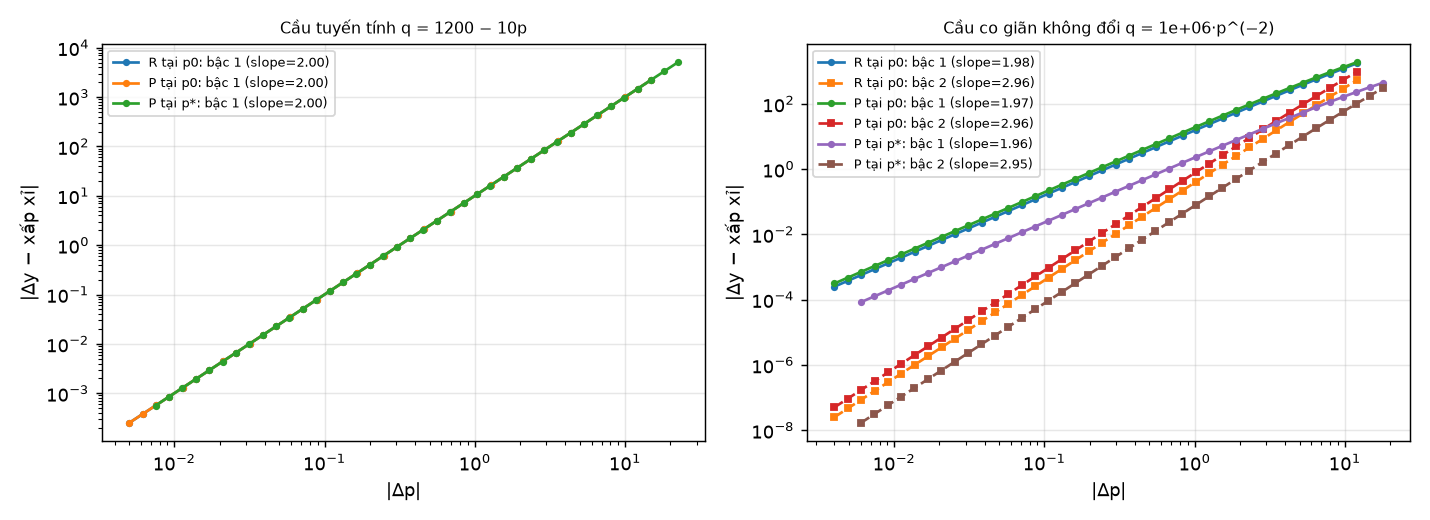
\includegraphics[width=\textwidth]{TN8_second_order_loglog.png}
\caption{Sai số của xấp xỉ bậc một và bậc hai theo $|\Delta p|$ (log-log).}\label{fig:tn8}
\end{figure}
